\documentclass[oneside]{book}

% Load the VUB package.
% This has many options, please read the documentation at
% https://gitlab.com/rubdos/texlive-vub
\usepackage{vub}

%href package to make references clickable.
\usepackage{hyperref}
\hypersetup{
    colorlinks,
    citecolor=black,
    filecolor=black,
    linkcolor=black,
    urlcolor=black
}

% Some highly suggested packages, please read their manuals.
\usepackage{cleveref}
\usepackage[natbib,style=apa]{biblatex}
\addbibresource{../bibliography.bib}
\usepackage{listings}
\usepackage{wrapfig}

%space between paragraph and indent all
\setlength{\parskip}{1em}
%\usepackage{indentfirst}

%quotes
\usepackage{epigraph}

%space between bib entries
\setlength\bibitemsep{2\itemsep}

%images settings
\graphicspath{ {./images/} }
\usepackage{graphicx,caption}
\usepackage{float}
\usepackage{rotating}
\usepackage{tikz}

% subfigures
\usepackage{subcaption}

% remove chapter text
\usepackage{titlesec}

\titleformat{\chapter}[display]
  {\normalfont\huge\bfseries}{}{0pt}{\Huge}
\titlespacing*{\chapter}
  {0pt}{10pt}{40pt}

%START title
\title{Computer generated car design}
\subtitle{Assignment 1 - Computational Creativity}
\author{Lennert Bontinck}
\date{February, 2020-2021}
\promotors{Student number: 568702}
\faculty{Computer Science: AI}
\begin{document}
\frontmatter
\maketitle
%END title

%START abstract
\chapter*{Abstract}

% OK

This paper discusses the development and evaluation of a creative system capable of generating photorealistic novel car designs and modifying them.
This system makes use of a pre-trained StyleGAN2 model \citep{stylegan2} and a modified version of the GANSpace tool \citep{ganspace}.
The various components are discussed loosely based on the computational creativity (CC) system description paper by \citet{ventura}.
These components are also placed inside the creative systems framework (CSF) proposed by \citet{csf} to further clarify the creative aspects of the system.

This paper also aims to discuss the possibilities and shortcomings of generative adversarial networks (GANs) in the CC field.
A more philosophical discussion is held to show such systems can indeed be creative rather than just generative.
It is shown how conceptual space exploration tools such as the modified GANSpace tool can be used to combat the black-box problems with GANs.
The need for CC specific internal evaluation and possible solutions are also briefly touched upon.
The external evaluation performed aims to further defend the creativity of the made system and thus the viability of GANs as a creative system.
The used tool for external evaluation was custom build for this project and is made available free to use and open source.

This paper was made as a requirement of the Computational Creativity course taught at the VUB.
All source files for this project are available on GitHub \citep{github_project}.
It is noted that this report is written using a modified version of the VUB based \LaTeX{} template from \citet{latex_template}. 
%END abstract


%TOC
\tableofcontents
\mainmatter

%START MAIN
\chapter{About the creative domain}
\label{ch:creative_domain}

% OK

In this chapter, the creative domain of car design is discussed.
Relevant literature in the CC field and surrounding GANs are briefly summarised.
The available resources for this project and the limits they bring with them are also touched upon.

%------------------------------------
\section{Car design and Computational Creativity}
\label{sec:why_car_design}

The car industry is only just over a century old and has already evolved from a motorized luxury carriage for the rich to a multi-billion euro industry for the masses.
In the last decade, the car industry has undergone major changes, with electrification and autonomous driving being the most prominent.
Computer algorithms play a key role in these changes to ensure safe autonomous driving and optimal battery usage.

However, computer algorithms do much more for the car industry.
They are used for crash test simulations \citep{crashtest}, automotive aerodynamics \citep{carearo} and more.
This raises the question: if the industry uses so many computer-generated simulations and calculations for validating the design of cars, can't a computer generate a car design?
This is a task that is gaining interest by big brands, especially in Formula 1 and hypercar design.

This paper explores that idea by building a creative system capable of generating photorealistic novel car designs and having control over the generated designs.
It is noted that the output of this system is only that, a picture of a car.
The true viability of the proposed car concerning legislation, safety and more are not taken into consideration. 
As is the case for architectural design, clothing design and many other design-related domains, car design is deemed a creative domain.
Some might argue against this idea, especially if they're not interested in cars.
Arguments could include that the limits put in place by legislation and the desire for reoccurring style traits of a brand limit the creativity in the domain.
Whilst many attempts at formalising what is (not) creative, such as the important work by \citet{boden2004creative}, have been made, it is still hard to objectively deem something creative.
However, with numerous car museums, legendary car design brands as Pininfarina and culturally driven evolution in car design, the domain is deemed creative for this paper.




%------------------------------------
\section{Relevant literature}
\label{sec:relevant_literature}

Much interesting relevant literature exists.
Some important papers on GANs and two relevant papers from the CC field are discussed in what follows.
These papers give better insight into how the technology used for this paper's system works and its viability as a useful creative system in the domain.

\subsection{Literature on GANs}
\label{subsec:relevant_literature_gan}

Generative adversarial networks (GANs), first introduced by \citet{gan_founder}, are systems capable of generating output images by training both a generator and discriminator to play a form of cat-and-mouse game.
More details on this idea are given later in this paper.
Such networks are the state-of-the-art used for image generation and have been used for similar, non-scientific, projects by \citet{gancar1}, \citet{gancar2}, \citet{gancar3} and more.
Many different variants of GANs exist, with an impressive recent example being BigGAN-deep by \citet{biggan}.
Perhaps the most known GAN is StyleGAN by \citet{stylegan}, researchers at NVidia.
It was used for a heavily media covered website that displays images of people who don't actually exist\footnote{\url{https://thispersondoesnotexist.com/}}.

For the system of this paper, a pre-trained StyleGAN2 model is used.
StyleGAN2 is a successor to the already mentioned StyleGAN \citep{stylegan2}.
StyleGAN2 introduces many improvements over the basic GAN idea by making use of concepts from the style transfer literature.
When trained on faces, the models seem to be capable of separating high-level attributes (e.g. orientation of face) and more low-level variations (e.g. presence of freckles).
Other differences include the use of four distinct random noise vector inputs to intermediate layers as opposed to only one starting noise vector with basic GANs.

Since StyleGAN and StyleGAN2 are made with the idea of being able to learn the concepts of an image, such as the discussed orientation and freckles with face generation, tools to easily control these parameters are being developed.
GANSpace by \citet{ganspace} is one of them.
GANSpace takes a trained model of either StyleGAN, StyleGAN2 or BigGAN and extracts interpretable controls for image synthesis of them.
This is done by identifying important latent directions based on PCA analysis in the activation space of these GANs.
The main contribution of this tool for this paper is that it allows exploration of a GANs conceptual space in an easy manner.


\clearpage
\subsection{Literature on car design in the CC field}
\label{subsec:relevant_literature_cc}

Some non-scientific projects that use GANs to generate novel car designs were already mentioned.
However, scientific papers on car design in the CC field aren't very common.
A particularly interesting research paper worth mentioning is the one by \citet{creativecargan}.
In their paper, a creative system is developed which takes a pen-and-paper sketch of a car and returns a graphical representation of what that car could look like in a more realistic representation.
The authors of that paper deem their system creative since it is capable of generating images from angles of the car that are not visible in the input sketch.

Their paper also demonstrates that creative systems can not only be used to complete a creative task but also as a source of inspiration for human-made creative work.
This is because, just like it is the case for this paper's system, their outputted images aren't meant to be viable or regulatory.
They are meant to give an idea of what a car based on their input sketch could roughly look like.
Moreover, their creative system proposes multiple variants based on the input sketch.
This allows the car designer to get inspiration for, and an idea of what a finalised design could look like.
The creative system is not made to replace a car designer's job, but rather to be a tool in optimising a car designer's workflow.

DARCI by \citet{darci} is a well-known system in the CC field that produce images through creative means.
DARCI is accepted as being a creative system in the field that makes use of neural networks (NNs).
Its use of NNs is important when discussing the viability of using GANs in the CC field later in this paper.



%------------------------------------
\section{Available resources}
\label{sec:available_resources}

GANs require a lot of images, often in the millions, to generate pleasing results.
Some of the pre-trained StyleGAN2 models made available by NVidia used over 20 million images for certain configurations \citep{stylegan2}.
Whilst it would be possible to create a web-scraper that gathers such a quantity of images from car auction websites, it isn't viable for this project.
This would mean an existing database of car images would need to be used for training the StyleGAN2 model.
One such database might be the LSUN-Stanford Car one by \citet{cardb}.
However, the amount of time required to train a StyleGAN2 model with this amount of data would be weeks, if not months with the computational power available for this paper.
Using fewer images and/or epochs would most likely result in non-viable results.
This is one of the reasons a pre-trained model is used.

For this paper, access to numerous experts in the car industry with excellent knowledge of existing car brands and models was available.
These people are seen as juries with expertise.
This helped tremendously to determine the P-creativity and H-creativity of the system, which is further discussed in the evaluation chapter of this paper.
\chapter{GANs and creativity}
\label{ch:generative_or_creative}

% OK

An important, but often difficult to answer, question in the CC field is whether a system is creative or simply generative.
To defend the claim of GANs being capable of becoming creative systems, the main idea behind them is first explained in a simplified manner.
The black box problem of GANs is discussed together with the challenges it forms.
This chapter concludes with a more philosophical take on why GANs can be creative systems.

%------------------------------------
\section{Main idea behind a GAN}
\label{sec:main_idea_GAN}

Figure \ref{fig:gan_explained} shows a visualisation of the different components of a GAN.
It becomes visible that there are two systems at play, a discriminator and a generator.
The discriminator has access to the database containing images of the concept the GAN should generate new instances for.
Its job is to either accept or reject an incoming image.
An image that is accepted can be seen as one that the discriminator finds to be of the concept it has learned and thinks it is not computer-generated.
In some instances, the discriminator is a continuous learning algorithm.
The generator learns by starting from a random noise vector and transforming it until it receives something accepted by the discriminator.
The main differences between different GAN technologies are the way how they implement the generator.


\begin{figure}[H]
    \centering
    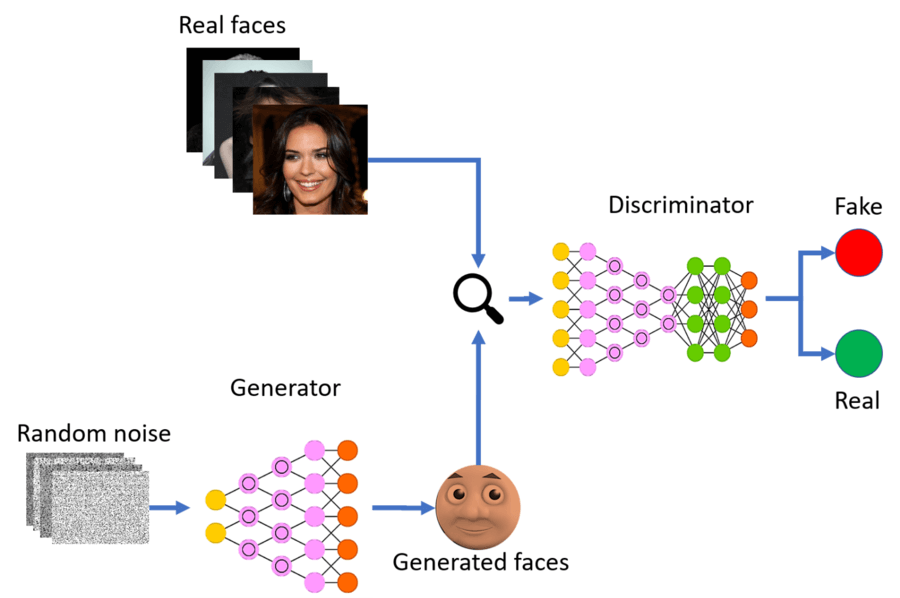
\includegraphics[width=0.55\linewidth]{images/gan_explained.png}
    \captionsetup{width=0.4\linewidth}
    \captionsetup{justification=centering}
    \caption{Basic idea of a GAN. Figure by \citet{howganworks}.  }
    \label{fig:gan_explained}
\end{figure}

%------------------------------------
\section{Black box problem}
\label{sec:back_box_problem}

One issue with GANs is that they almost always make use of deep NNs for both their generator and discriminator.
A deep NN is known to be a black-box model.
This means that there is no meaningful insight on how the model works, it is just a bunch of mathematical manipulations a human cannot reason about.
This makes it hard to state that a deep NN has learned something.
One can only evaluate if the output is what is desired.
This introduces the risk of claiming that you think a deep NN has learned something whilst in reality it might have learned something completely different which happens to give the same desired output by chance.
This is an important issue for AI in general.
An academic example that is often given to demonstrate this point is one where a tank recognition NN didn't learn to differentiate trees and tanks but rather the time of the day, which happened to correspond with the presence of tanks for the training and test samples.
Whilst this example demonstrates the issue at hand, it is noted that it could be an urban legend as discussed in a blog post by Gwern Branwen \footnote{\url{https://www.gwern.net/Tanks}}.


%------------------------------------
\section{GANs as creative systems}
\label{sec:GAN_as_creative}

In the CC field, understanding the process for achieving an output that might be deemed creative by humans is an important manner in deeming a system creative.
This makes algorithms with the black box problem such as GANs a hard case for creative systems.
However, the discussed DARCI system by \citet{darci} shows that systems using NNs can indeed be deemed creative if defended appropriately.
One of the convincing strengths of DARCI is that it gives a natural language description of the steps it takes to generate an image.
These are things such as explaining what image of the training set it relates to and what the labels for that known image are.
These descriptions aim to give an insight into the process of the creative system to try and tackle the black box problem.
However, DARCI does not know the semantic meaning of those descriptions and labels.
All of the natural language descriptions and labels were provided by a human as training data and statistically processed by the system.
It is even very likely that the internal representation of those strings is numerical through encoding.
Knowing this, the natural descriptions it delivers are likely to give the false perception that the system has a sense of semantic reasoning, which it does not.
It also gives a wrong idea of how the generative process of the system works.

Not all is bad though, as is mentioned in the paper on how to build a CC system by \citet{ventura}, some argue that not knowing what aesthetic the system is using is a positive advance as it gives more freedom and thus enhances creativity.
Whilst it would be easy to just agree with this as a defence on why explainability shouldn't be of huge concern for the CC field, there are some issues with this.
First of all, Ventura is a co-author of the older DARCI system.
Since DARCI uses NNs, Ventura couldn't suddenly state explainability are a must for creative systems, as that would render DARCI a non-creative system.
His use of GANs as examples in the paper further shows his stance on this topic.
However, one of the three characteristic Ventura gives to computationally creative agents is intentionality.
To defend intentionality correctly, a certain idea of how the generative process works needs to be present.
Explainability is also something that is desired for scientific fields in general.

\clearpage
So, where does this leave GANs as (part of) a creative system?
As it turns out, the days of true black-box models, where no analysis on learned concepts was performed, seem to have passed.
This is mainly due to new regulations being hard on the explainability of AI algorithms. 
Since deep NNs are often the desired solution for AI problems, much research in making them explainable is being done.

Papers such as the one by \citet{invidualunitanalysis} have an interesting approach to enhance explainability.
They analyse the meaning of individual units of a deep NN by disabling or boosting their output.
From this, they conclude multiple things.
One example is the detection of units that are responsible for generating trees, as disabling them drastically lowers the generation of trees and vice versa.
These approaches are steps in making it more defensible that a deep NN has indeed learned certain concepts.
This leads to why tools such as GANSpace can aid in the explainability of a GAN.
It also gives an insight into the generation process of the GAN and thus the use of GANs in the CC field becomes more viable.
If it is possible to determine components within one or more layers of the GAN to be responsible for the creation of distinct concepts in hundreds of samples, can it then not be claimed the system has learned that concept?
When does luck become skill?
On the GitHub repository for this paper, multiple examples of changing distinct concepts through GANSpace can be found.
Some are also discussed in the evaluation chapter of this paper and shown in figure \ref{fig:groupedsurvey}.
From this, it becomes clear the system does have an explainable generation process that consists of generating multiple distinct concepts to form a final image.

Once the above statements about the GAN's generation procedure are accepted, it's an easier step towards claiming them creative systems.
In the discussed internal working of a GAN, it is visible that internal evaluation is a crucial part of the design already.
GANs are also more than just an optimisation problem, as there is no "best image to generate", much as there is no "best artwork to generate".
Since the generator doesn't have direct access to the dataset and uses random noise vectors as its input it becomes clear it is creating things from the knowledge it has learned through the discriminator.
From the above statements, it becomes clear that knowledge is indeed meaningful concepts rather than random values.
The training loop then limits the conceptual space of the generator from all possible combinations of pixels to all images accepted by the discriminator.
This process corresponds to the generator becoming better at understanding the different concepts a car design requires.

One of the only challenges remaining to deem GANs creative is whether or not the created images are different enough from existing cars.
A reverse image search analysis, such as the ones used by Google reverse image search, can be used to ensure novelty.
Most of such state-of-the-art algorithms for this task also use deep NNs.
A recent paper by \citet{reverseimagesearch} discusses how such behaviour could be reached by using a pre-trained convolutional NN.
It is noted that adding such an evaluation metric would only ensure P-creativity, as it only has access to the training images and not all cars ever made.
It is also important to remember from the domain explanation that similarity to existing models is expected and often even desired in car design.
Thus, for this specific domain, there should possibly even be a lower bound for this similarity metric.
Having hyper-parameters for these thresholds is recommended.
With this final required component of the system in place, it can be seen that GANs can indeed be creative systems.
\chapter{Design of the system}
\label{ch:design_of_system}

% OK

Backed by relevant literature and a more philosophical take on how GANs can be deemed creative systems, the design of the system is discussed in this chapter.
The working of the various components is presented loosely based on the CC system description paper by \citet{ventura}.
These components are also placed inside the creative systems framework (CSF) proposed by \citet{csf} to further clarify the creative aspects of the system.

%------------------------------------
\section{Overview of the system}
\label{sec:overview_system}

\begin{figure}[H]
    \centering
    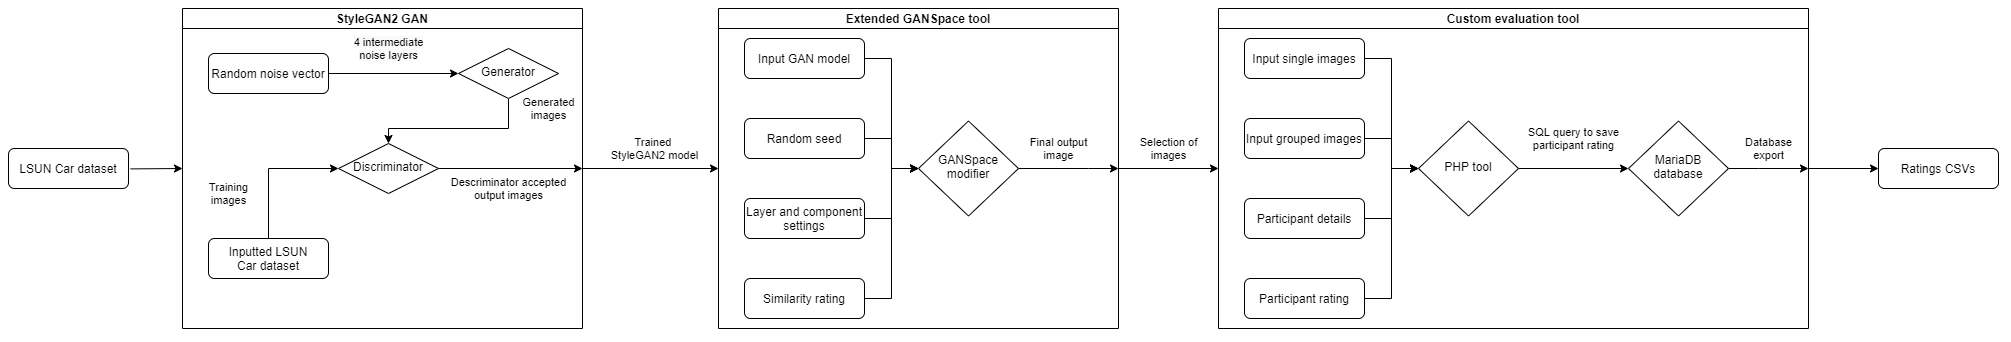
\includegraphics[width=\linewidth]{images/system_overview.png}
    \captionsetup{width=0.7\linewidth}
    \captionsetup{justification=centering}
    \caption{ High level overview of whole creative system's pipeline including external evaluation.  }
    \label{fig:system_pipeline}
\end{figure}

The whole pipeline of the developed system is visualised in figure \ref{fig:system_pipeline}.
For this paper, the first step of training the StyleGAN2 model is bypassed by using a pre-trained one.
The StyleGAN2 car pre-trained model with configuration f is used.
This model generates images of cars at a resolution of 512 by 384 pixels.
It used the LSUN Car dataset for training, which is part of the discussed LSUN-Stanford Car dataset by \citet{cardb}.
It was the highest resolution pre-trained car model at the time of writing.
With the use of an NVIDIA DGX-1 with 8 Tesla V100 GPUs, it took 4 days and 18 hours to train \citep{stylegan2}.
The different components of the extended GANSpace tool, as well as the custom evaluation tool, are discussed later in this paper.

It becomes clear all of the steps and components proposed by \citet{ventura} are in place.
As already discussed, the domain of car design is chosen.
Car design is represented by a phenotypic representation of images of cars.
Internally the genotypic representation of these images is a numerical vector representing the images.
Their exact representation is StyleGAN2 specific.

The used data is the LSUN Car dataset which through conversion to the genotypic representation is used as the knowledge base by the discriminator of the GAN.
The generator function is the generator of the GAN which makes use of four intermediate random noise vectors and more as "input".
More technical details on this can be found in the StyleGAN2 paper \citep{stylegan2}.
Multiple aesthetic measures exist such as the inclusion of required car components, appearance of car brand styling traits and more.
These are mainly taken care of by the discriminator which serves as the value measure.
The similarity rating serves as the novelty measure.
The external evaluation serves as the phenotypic evaluation.

%------------------------------------
\section{Defending the design decisions}
\label{sec:defending_design}

Due to the discussed available resources being rather limited, a pre-trained StyleGAN2 model was the only feasible choice.
The similarity rating is done manually due to limited resources as well, this is further explained later in the paper.
These made design decisions don't limit the creative system of this paper but give rise to interesting future extensions, which are discussed at the end of this paper.

%------------------------------------
\section{Putting it in terms of the CSF}
\label{sec:csf}

A presentation where the system is situated in terms of the CSF was given at the VUB and the used slides are available under the presentations folder of the GitHub repository for this paper \citep{github_project}.
A summary of the contents is given below.
Many different frameworks for describing creative systems exist.
The CSF is chosen as it is formalised the concepts introduced by \citet{boden2004creative} and is created by \citet{csf}, two of the founding figures of CC.
\begin{itemize}
    \item The universe $U$ is Technically all RGB combination of pixels. For the generator, this boils down to all images deemed “real” by the discriminator. When assuming the discriminator does its job, the universe thus consists of all images of realistic-looking cars.
    \item The conceptual space $C$ is the set of all images the generator can make based on all possible noise vectors using its latest transformers. It is clear that $ C \subset U$
    \item Remember from the CSF that $C = [[R]](U)$. This means the rules $R$ constraining the space are the same rules defining the state of the generator.
    \item The rules $T$ are those that introduce randomness and noise as restrictions on the latent spaces. At a high level, the extended GANSpace tool uses these rules to explore the conceptual space.
    \item The rules $E$ are those that define the discriminator as they can be used to assess the quality of the generated image. The similarity rating also belongs to these rules. To keep the language $L$ unchanged, it should be implemented in the same language being a combination of Python and C++.
    \item Since $F^\diamondsuit$ is limited by the output of images having 512 by 384 pixels it is finite. This means $e_c = <R, T, E>^\diamondsuit(\{T\})$ is also finite. Since GANSpace could bypass some of StyleGAN2's rules it is possible that $e_c \not\subset C$.
\end{itemize}
\chapter{Implementing the creative system}
\label{ch:implementation}

% OK

This chapter goes over the technical details of the implementation of the system.
Firstly, the used pre-trained StyleGAN2 model \citep{stylegan2} is discussed. 
The issues with and extensions made to the GANSpace tool \citep{ganspace} are also explained here.
Since the GANSpace tool lacks documentation and support, special attention has been taken to ensure reproducibility.

%------------------------------------
\section{Using StyleGAN2 model}
\label{sec:sytelgan2_implement}

Using a pre-trained StyleGAN2 model is easy and doesn't require an extraordinary amount of computational power.
As StyleGAN2 is created by researchers at NVidia, it's recommended to have an NVidia GPU, especially one with CUDA support.
These are widely available and the system used for this project had a relatively old GTX 970 with 4 GB of VRAM.
With just a few lines of Python code and the download of a pre-trained model, which is about 1 GB in size, the GAN is loaded in and starts generating images.
The generation of a singular image takes seconds at most for the GTX 970 system.
Google's Colaboratory Notebooks are also capable of doing just this with the free tier.
Since downloading and starting the pre-trained model is taken care of automatically by the extended GANSpace tool, no further instructions are given.

%------------------------------------
\section{Extending the GANSpace tool}
\label{sec:GANSpace_implement}

Whilst GANSpace is an incredibly easy tool to gain interpretable control over a GAN with, it does have some shortcomings and flaws.
As a starter, the documentation isn't up to par and due to the low popularity, troubleshooting isn't an easy task.
The installation guide at the time of writing lacks crucial steps such as specifying all required dependencies and more.
Support for anything other than Linux distributions is poor.
Because of this, it was chosen to create a fresh install of Ubuntu 20.04 and document all steps required to get the tool to work.
These steps and much more documentation are available on the GitHub repository of this project \citep{github_project}.
The new setup guide is available under the GANSpace folder as SETUP.md, it is also published to the issues page of the GANSpace tool\footnote{\url{https://github.com/harskish/ganspace/issues/49}}. The used Pycuda folder is also made available.

Besides this, a simple script called rungan.sh is made, which upon execution initializes the GANSpace environment exactly as it was used for this paper.
After successfully running this script, a screen as shown in figure \ref{fig:extended_ganspace_tool} should be presented.
Note the visual queues such as the setting field being set to 'Creative Car Design' and the title of the window being custom for the project.
The most important added feature is the possibility of saving the canvas.
This works for all possible batch sizes.
The code responsible for generating different images after resampling the latent space is also discussed inside the exploring\_GANSpace.md file under the GANSpace folder.
This is important for the similarity measure as is discussed in the evaluation chapter of this paper.


\begin{figure*}
\centering
\begin{subfigure}{.5\textwidth}
  \centering
  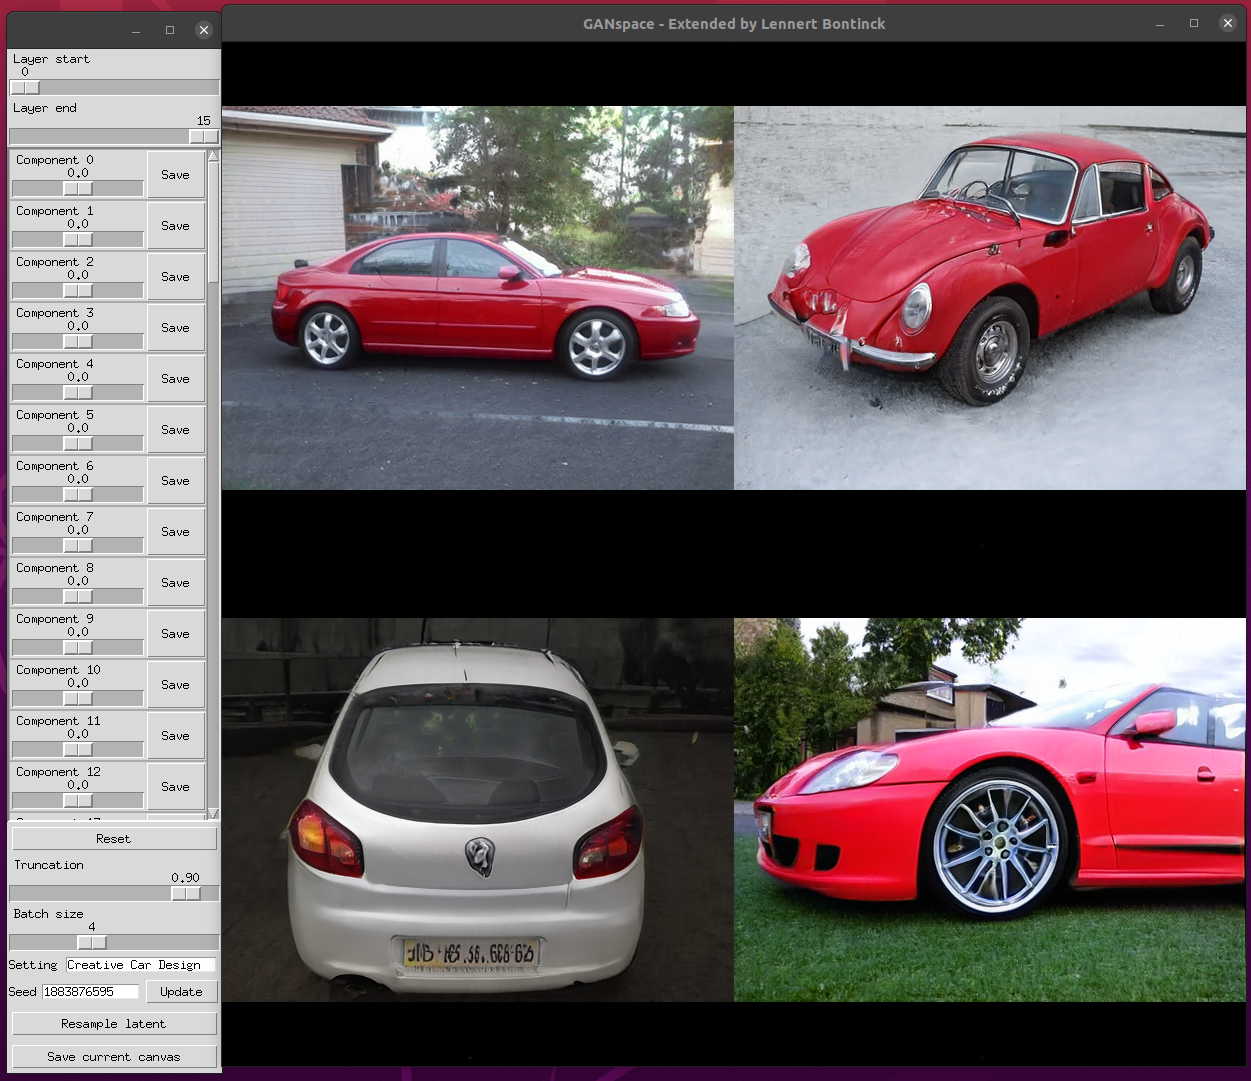
\includegraphics[width=\textwidth]{images/extended_ganspace.png}
  \caption{Extended GANSpace tool}
  \label{fig:extended_ganspace_tool}
\end{subfigure}%
\hspace{1cm}
\begin{subfigure}{.4\textwidth}
  \centering
  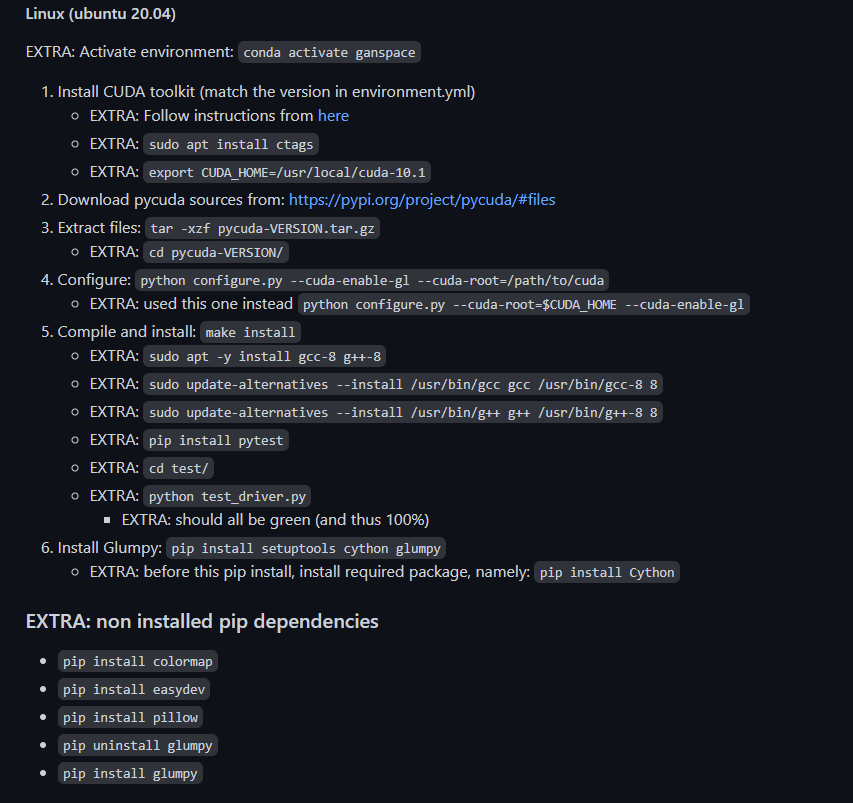
\includegraphics[width=\textwidth]{images/documentation.PNG}
  \caption{Exhaustive documentation}
  \label{fig:extended_ganspace_doc}
\end{subfigure}
\captionsetup{width=.85\linewidth}
\caption{Screenshot of the extended GANSpace tool and documentation.}
\label{fig:extended_ganspace}
\end{figure*}


%------------------------------------
\section{Reproducibility}
\label{sec:reproducibility_implement}

In contrast with the original GANSpace tool documentation, this project contains all required details on downloading and running all required dependencies and code.
The custom made script that was discussed allows for a one-line command to initialize the GANSpace tool identically to the one used.
It downloads the discussed pre-trained StyleGAN2 model automatically. 
All of the settings for generated images and found modifications are also written down.
These are documented in the exploring\_GANSpace.md file under the GANSpace folder as well as the README.md of the generated images folder.
This means that by simply setting the seed and changing the corresponding sliders as documented, identical results can be achieved.
\chapter{Evaluation}
\label{ch:evaluation}

% OK

Perhaps the most important part of a creative system is evaluation, both internally as external.
This chapter goes over both.
Due to the limited resources, internal evaluation is non-optimal but solutions are proposed.
Some of the reoccurring issues with the system's output are also discussed.
A heavy focus was put on the external evaluation and a custom build evaluation tool was made.
How this tool works and the results of the external evaluation are discussed here.

%------------------------------------
\section{Internal evaluation}
\label{sec:internal_evaluation}

As was already discussed, the discriminator is responsible for automatic internal evaluation.
The generator can use it to assess the quality of the generated image by either being accepted as real or not.
However, the point was raised that it is not possible to validate whether the generated images differ enough from existing cars.
If the discriminator is too strict, the generator can end up generating nearly identical images to the one in the training set.
Such a system would produce incredibly realistic results but is hard to call creative.
Currently, StyleGAN2 and other state-of-the-art models don't seem to have a metric in place to strictly evaluate this behaviour.

However, as was already discussed, a solution for this problem exists in the form of a reverse image search analysis.
Due to limited resources for this paper, this was not implemented.
However, the documentation on where the generation of new images occurs in the extended GANSpace tool is discussed.
This allows for future extensions where an automatic evaluator can be made to skip the output of the StyleGAN2 model that resembles a car from the training set too much.
It is noted that this ideology was used in the selection of images for evaluation, where three domain experts sat together to discuss which cars they recognized.
These experts were a Peugeot car mechanic, a Mercedes sales manager and a Honda employee. 
From this, a selection similar to the use of such an evaluation metric was made.
It is also important to note that providing this metric inside GANSpace would make it a wrapper function, meaning, the actual training of the model remains unchanged.
In an ideal world, this evaluation metric would be built into the used GAN technology.

Finally, the extended GANSpace tool helped validate the GAN has indeed learned concepts related to car design by using the same reasoning as the discussed paper by \citet{invidualunitanalysis}.
The generation process thus consists of making an image that contains learned concepts of a car.
Since the generated car designs are different enough from existing cars, they can be deemed creative in a similar manner \citet{creativecargan} deemed their system creative.



%------------------------------------
\section{Challenges for the GAN}
\label{sec:challenging_angle}

\begin{figure*}
\centering
\begin{subfigure}{.3\textwidth}
  \centering
  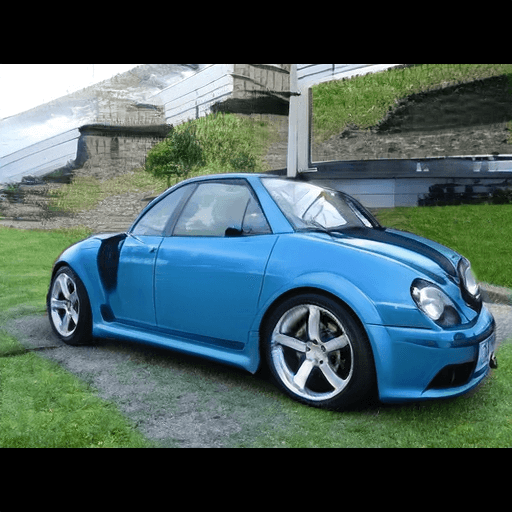
\includegraphics[width=\textwidth]{images/double_front.png}
  \caption{Double front car}
  \label{fig:doublefront}
\end{subfigure}%
\hspace{.02\textwidth}
\begin{subfigure}{.3\textwidth}
  \centering
  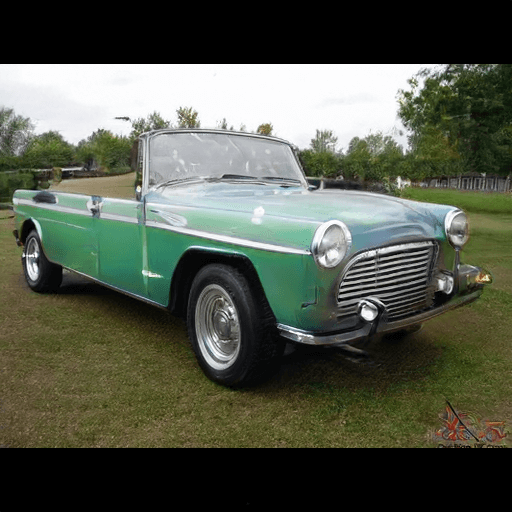
\includegraphics[width=\textwidth]{images/missing_piece.png}
  \caption{Missing piece in bed}
  \label{fig:missingpiece}
\end{subfigure}
\hspace{.02\textwidth}
\begin{subfigure}{.3\textwidth}
  \centering
  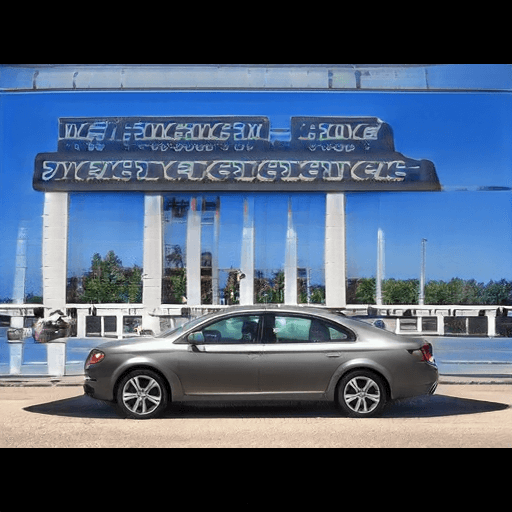
\includegraphics[width=\textwidth]{images/text.png}
  \caption{Attempt at text}
  \label{fig:textattempt}
\end{subfigure}
\captionsetup{width=.85\linewidth}
\captionsetup{justification=centering}
\caption{Multiple images generated by the system that demonstrate some of its flaws. Settings and more info available on GitHub \citep{github_project}.}
\label{fig:challanging_angle}
\end{figure*}

Whilst analysing the output of the GAN, it became visible the GAN had some reoccurring issues with its generated images.
One of these issues is what the documentation available on GitHub calls the 'challenging' angle.
When looking at the car from an angle in between front and side, the GAN seems to confuse what is front and back.
This results in realistic images of cars that have two fronts or two backs.
One such example is shown in figure \ref{fig:doublefront}.

Another challenge seemed to be that the GAN didn't always seem to generate the car in all dimensions.
This is shown in figure \ref{fig:missingpiece}, where a piece of the bed on the pick-up and convertible crossover is missing and replaced by grass.
Including images where such dimensions are missing might be interesting for the external evaluation to get an idea if participants notice it. 

The final reoccurring issue that is worth mentioning, is the system's poor performance in generating realistic backgrounds.
Whilst generating static backgrounds such as grass and trees was pretty successful most of the time, generating more complex environments often failed.
It could be argued this is a good thing, as it means the discriminator and generator have a focus on the realism of the car, which is the purpose of this system.
One of the most interesting phenomenons with background generation was the system's attempt at generating text.
An interesting example of this is shown in figure \ref{fig:textattempt}.

Other reoccurring anomalies from regular car designs were also noticed.
One such example is the fact that the headlight design was different on the other side of the car.
Whilst this is (almost) never found in car designs presents, it's not seen as an "issue of the GAN".
Besides this, the generated cars are often relatively symmetrical.
It is noted that the GAN also produced some outlandish results from time to time.
However, this was less than 10\% over more than 500 samples.
One such artefact is shown in figure \ref{fig:survey_creative_artefact}.



%------------------------------------
\clearpage
\section{Making a suitable external evaluation tool}
\label{sec:external_evaluation_tool}

\begin{figure*}
\centering
\begin{subfigure}{.3\textwidth}
  \centering
  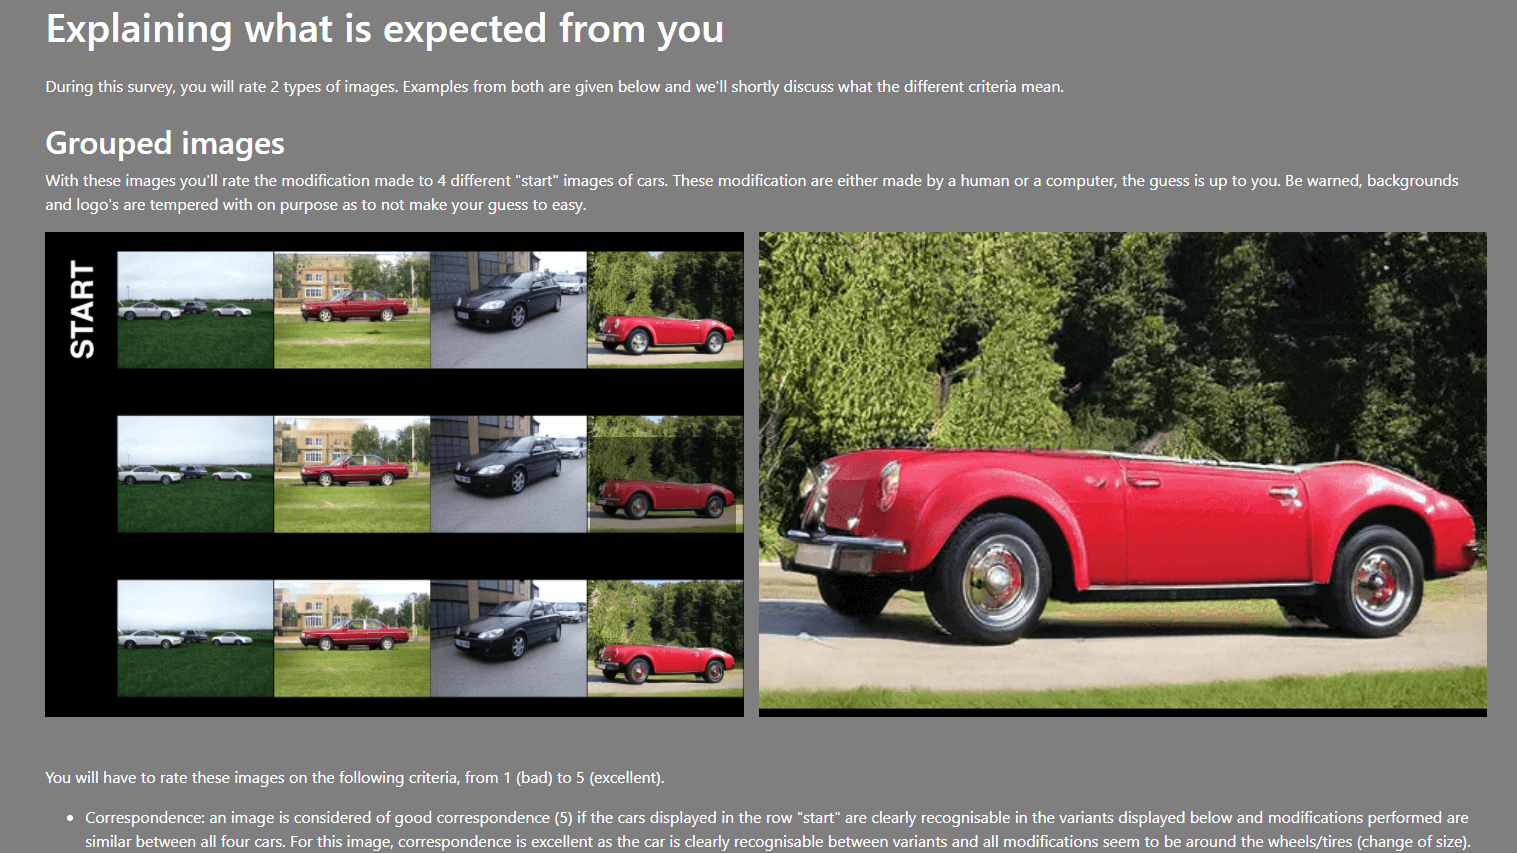
\includegraphics[width=\textwidth]{images/survey1.PNG}
  \caption{Explanation of survey}
  \label{fig:explain_survey}
\end{subfigure}%
\hspace{.02\textwidth}
\begin{subfigure}{.3\textwidth}
  \centering
  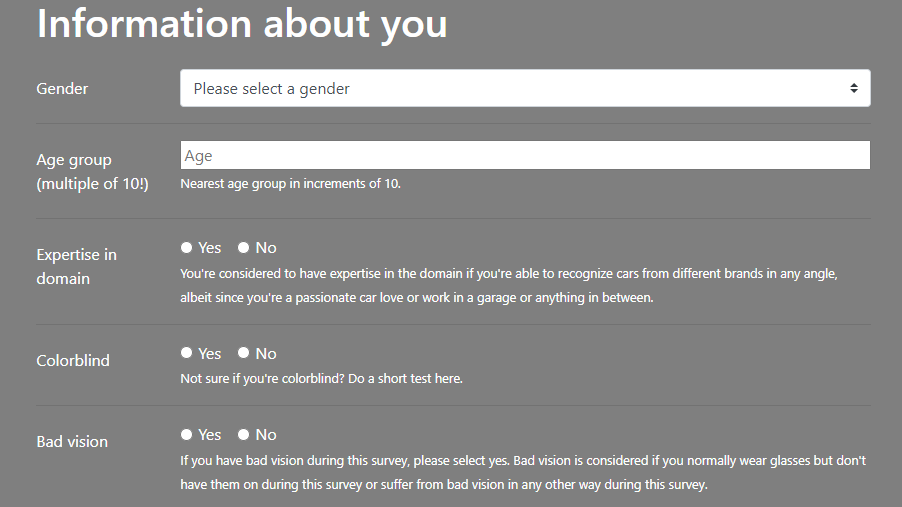
\includegraphics[width=\textwidth]{images/survey2.PNG}
  \caption{Personal information}
  \label{fig:personal_info_survey}
\end{subfigure}
\hspace{.02\textwidth}
\begin{subfigure}{.3\textwidth}
  \centering
  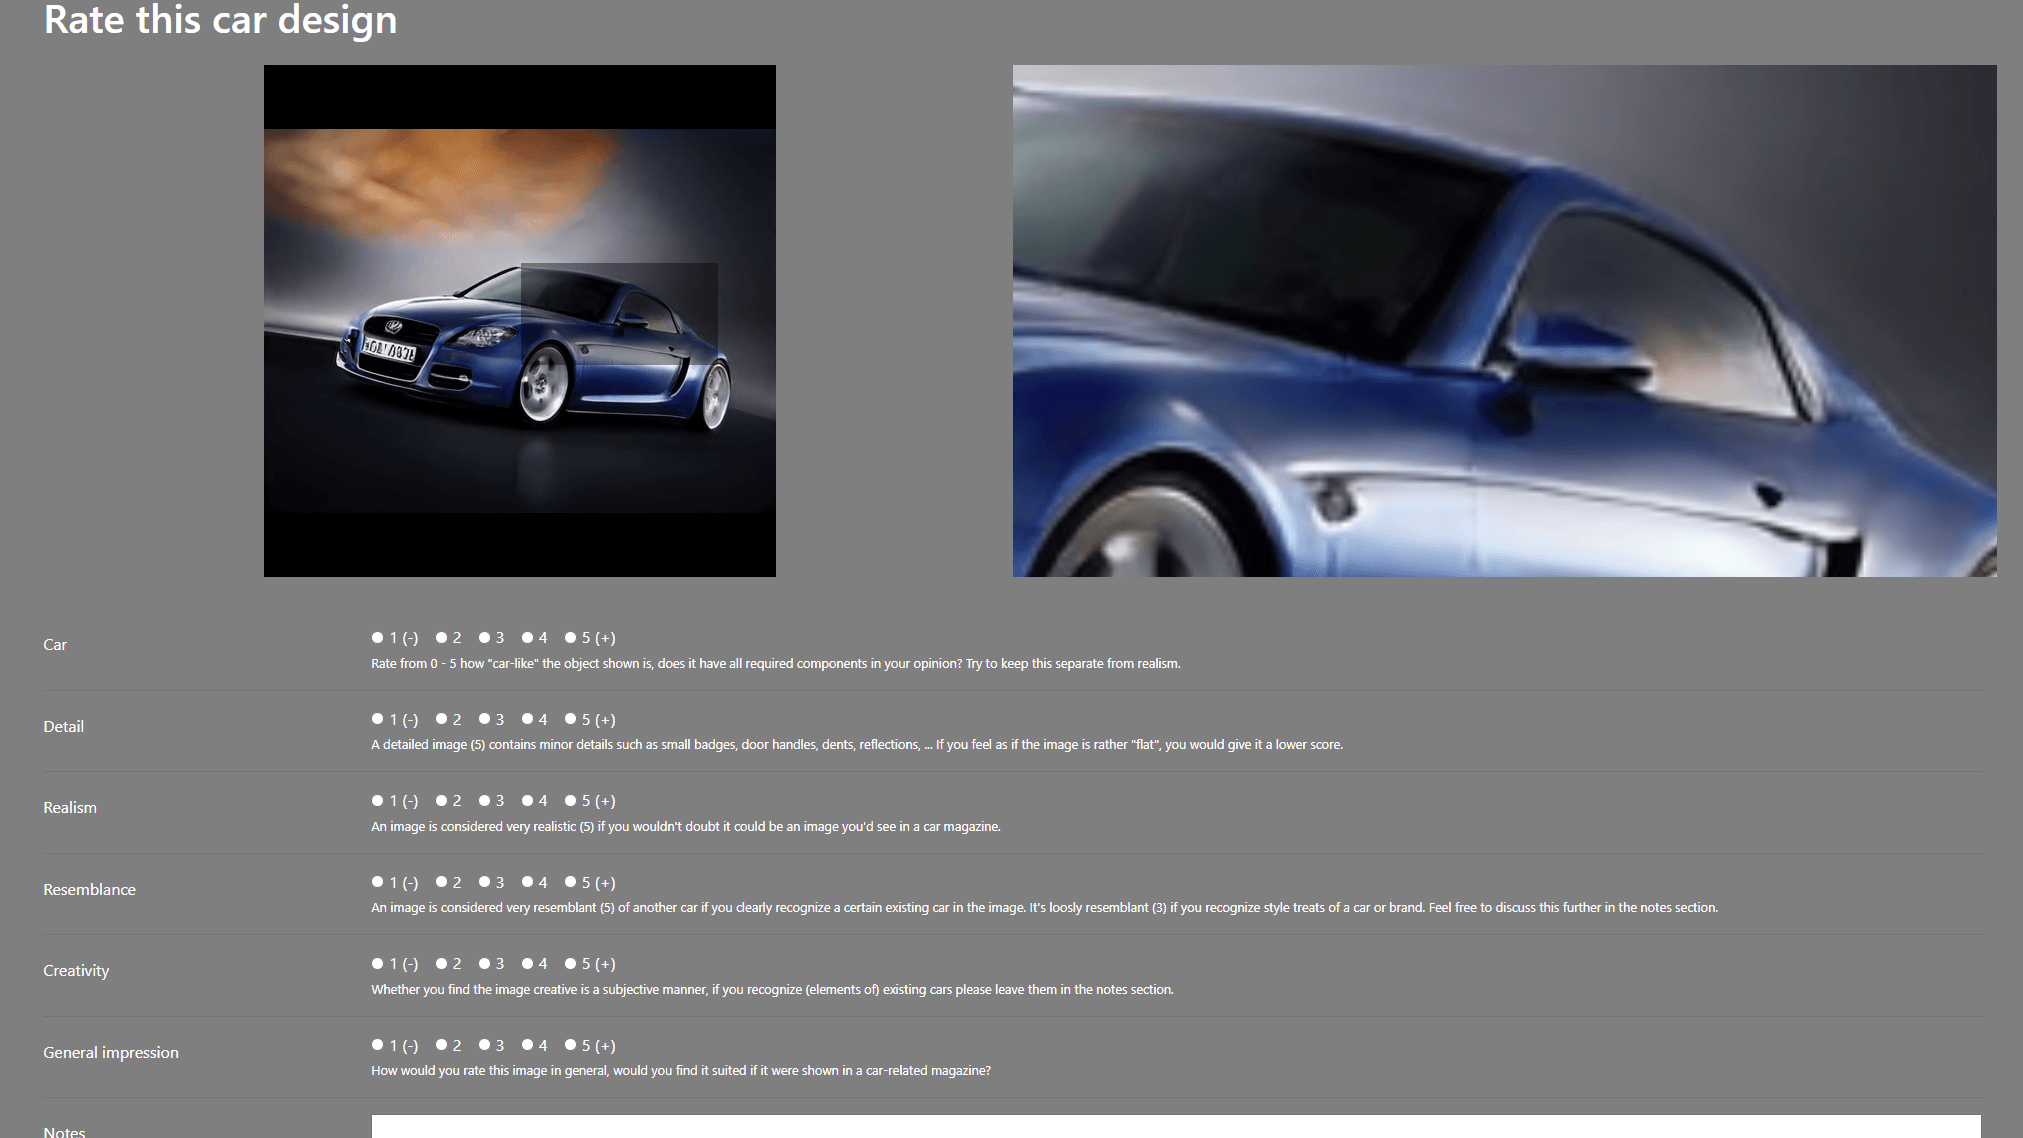
\includegraphics[width=\textwidth]{images/survey3.PNG}
  \caption{Single image rating}
  \label{fig:single_survey}
\end{subfigure}
\captionsetup{width=.85\linewidth}
\captionsetup{justification=centering}
\caption{Screenshots of the created external evaluation tool.}
\label{fig:survey}
\end{figure*}


This paper aimed to make a creative system capable of generating photorealistic novel car designs.
The external evaluation helps in proving this goal is reached.
To ensure proper evaluation, a custom made PHP based survey tool is made.
This tool is based on a previous project from the author of this paper \citep{bapproef}.
Some screenshots of the tool, which was made available online\footnote{\url{https://www.lennertbontinck.com/creative-car-design-survey/}}, are shown in figure \ref{fig:survey}.
The flow of the system is described below.
\begin{itemize}
    \item Initialize the evaluation tool by visiting setup.php using the chosen key. This will create all required SQL tables and insert the images from the images folder into the images table. This step has to be performed only once.
    \item Participants can now complete the survey by navigating to the index.php web page.
    \item Show participant what personal information will be collected and what the survey is about.
    \item Show a more detailed explanation of all fields that need answering (see figure \ref{fig:explain_survey}):
    \begin{itemize}
        \item Explains some images are made by a computer algorithm and others by a human through photo editing software.
        \item Explains the backgrounds and logos have been tampered with on purpose to make the above choice harder. This is done due to the issues the GAN has with more complex backgrounds as described earlier.
    \end{itemize}
    \item Ask the user some personal information (see figure \ref{fig:personal_info_survey}):
    \begin{itemize}
        \item Gender (optional) and age in multiple of 10. The latter is done to improve anonymity. 
        \item Expertise: Participant is considered to have expertise in the domain if he is capable of recognizing cars from different brands from any angle.
        \item Whether the participant is colour blind or has other vision issues when taking the survey (e.g. not wearing glasses).
    \end{itemize}
    \clearpage
    \item Show two grouped images and four single images. These are selected at random from the evaluation set.
    \begin{itemize}
        \item Grouped images are images where the GANSpace tool is used to perform modifications. The following criteria are asked using a Likert scale from one to five:
        \begin{itemize}
            \item Correspondence: an image is considered of good correspondence (5) if the cars displayed in the row "start" are recognisable in the variants displayed below and modifications performed are similar between all four cars.
            \item Realism: an image is considered very realistic (5) if it could be an image from a car magazine.
            \item Creativity: Subjective measure, recognition of (elements of) existing cars can influence this.
            \item Made by: Whether participant thinks the modifications are made by a human or a computer.
            \item Notes: field for the participant to leave notes such as recognized cars.
        \end{itemize}
        \item Single images are images straight out of the StyleGAN2 model, taking into account the selection done using the similarity measure. The following criteria are asked using a Likert scale from one to five:
        \begin{itemize}
            \item Car: how "car-like" the object shown is, does it have all required components etc.
            \item Detail: a detailed image (5) contains minor details such as small badges, door handles, dents, reflections, ... If the image is rather "flat", it would receive a lower score.
            \item Realism: same ideology as before.
            \item Resemblance: an image is considered very resemblant (5) of another car if the participant recognizes a certain existing car in the image. It's loosely resemblant (3) if he recognizes the style treats of a car or brand.
            \item Creativity: same ideology as before.
            \item General impression: how the participant would rate this image in general.
            \item Made by: same ideology as before.
            \item Notes: same ideology as before.
        \end{itemize}
    \end{itemize}
    \item Show the participant a screen admitting he's been lied to and all images have been computer-generated. Ask whether or not the participant thinks he was biased.
    \item Similarly show the other evaluation images. The "made by" field is now automatically set to "known".
    \item Export all SQL tables to CSV files by navigating to the export.php web page using the chosen key.
\end{itemize}

The tool is made available under the GPL V3 license and is available with documentation on the GitHub repository of this project \citep{github_project}.
On the same GitHub page, all used images for the external evaluation and the documentation to reproduce them is also available.
Some of the images generated through GANSpace modifications were minor changes such as different wheel designs whilst others were major changes such as making a car look more sporty.
These are displayed in figure \ref{fig:groupedsurvey}.
The single images contained various examples, from super realistic examples to creative artefacts of the system.
Some are shown in figure \ref{fig:singlesurvey}.


\begin{figure*}
\centering
\begin{subfigure}{.3\textwidth}
  \centering
  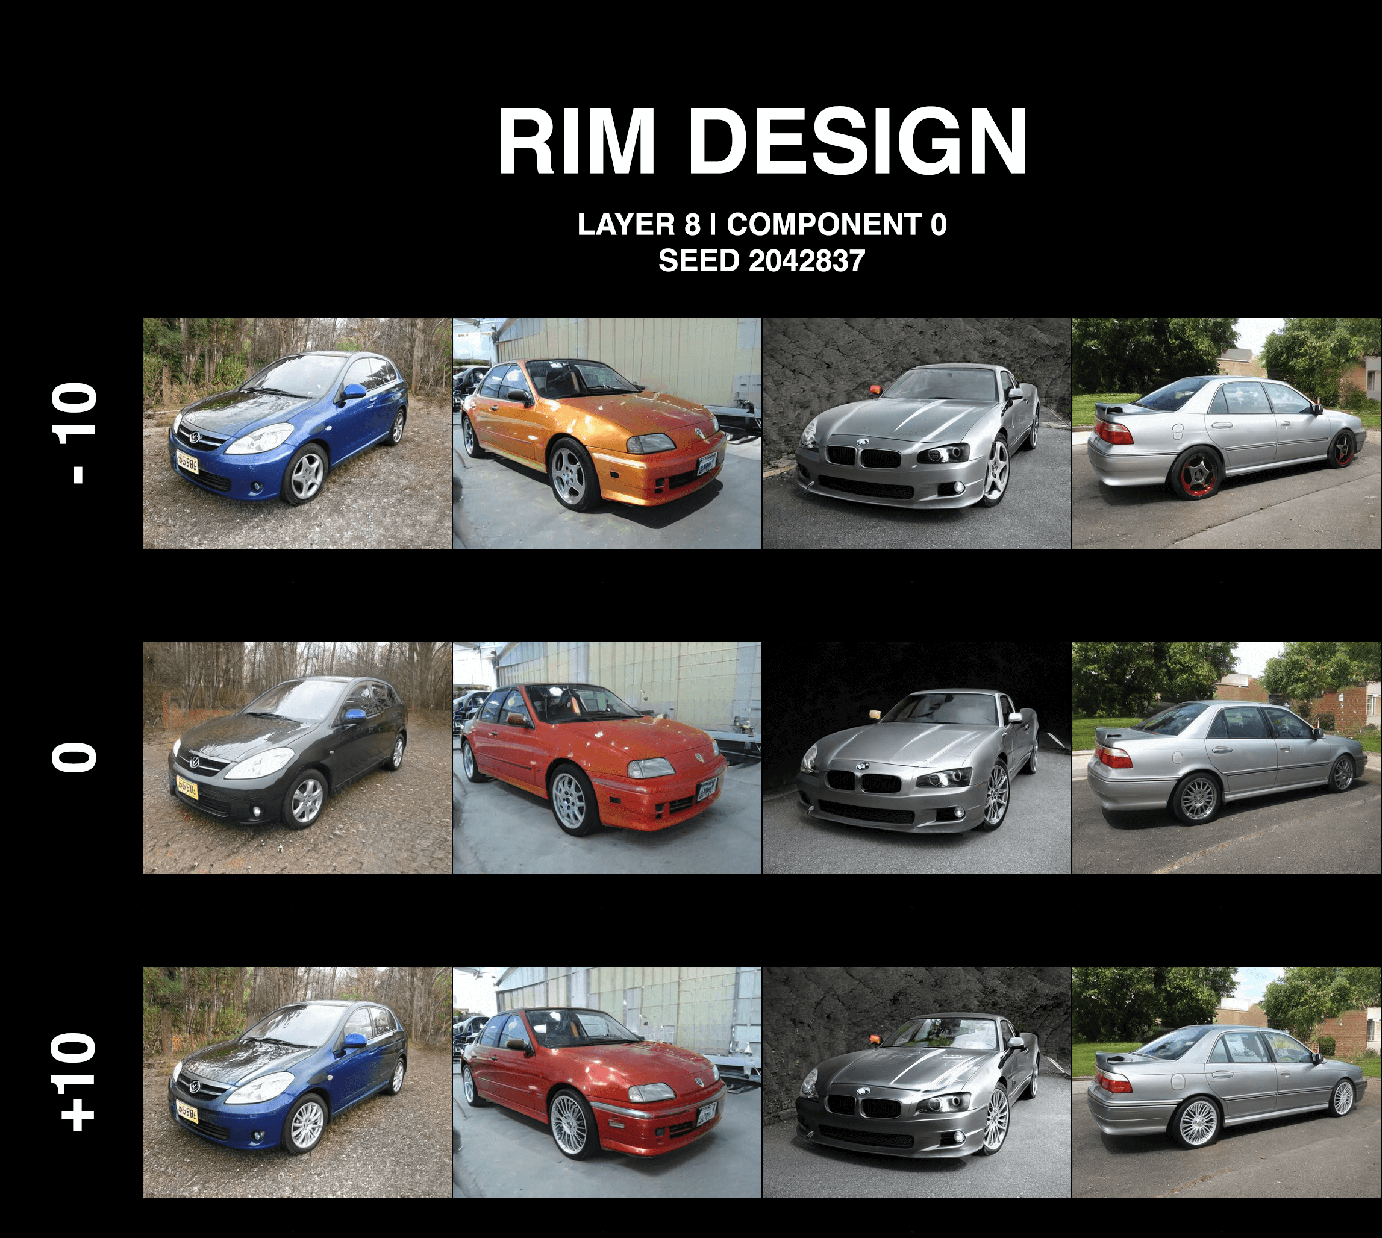
\includegraphics[width=\textwidth]{images/rim_design.pdf}
  \caption{Minor edits}
  \label{fig:rimdesign}
\end{subfigure}%
\hspace{.02\textwidth}
\begin{subfigure}{.3\textwidth}
  \centering
  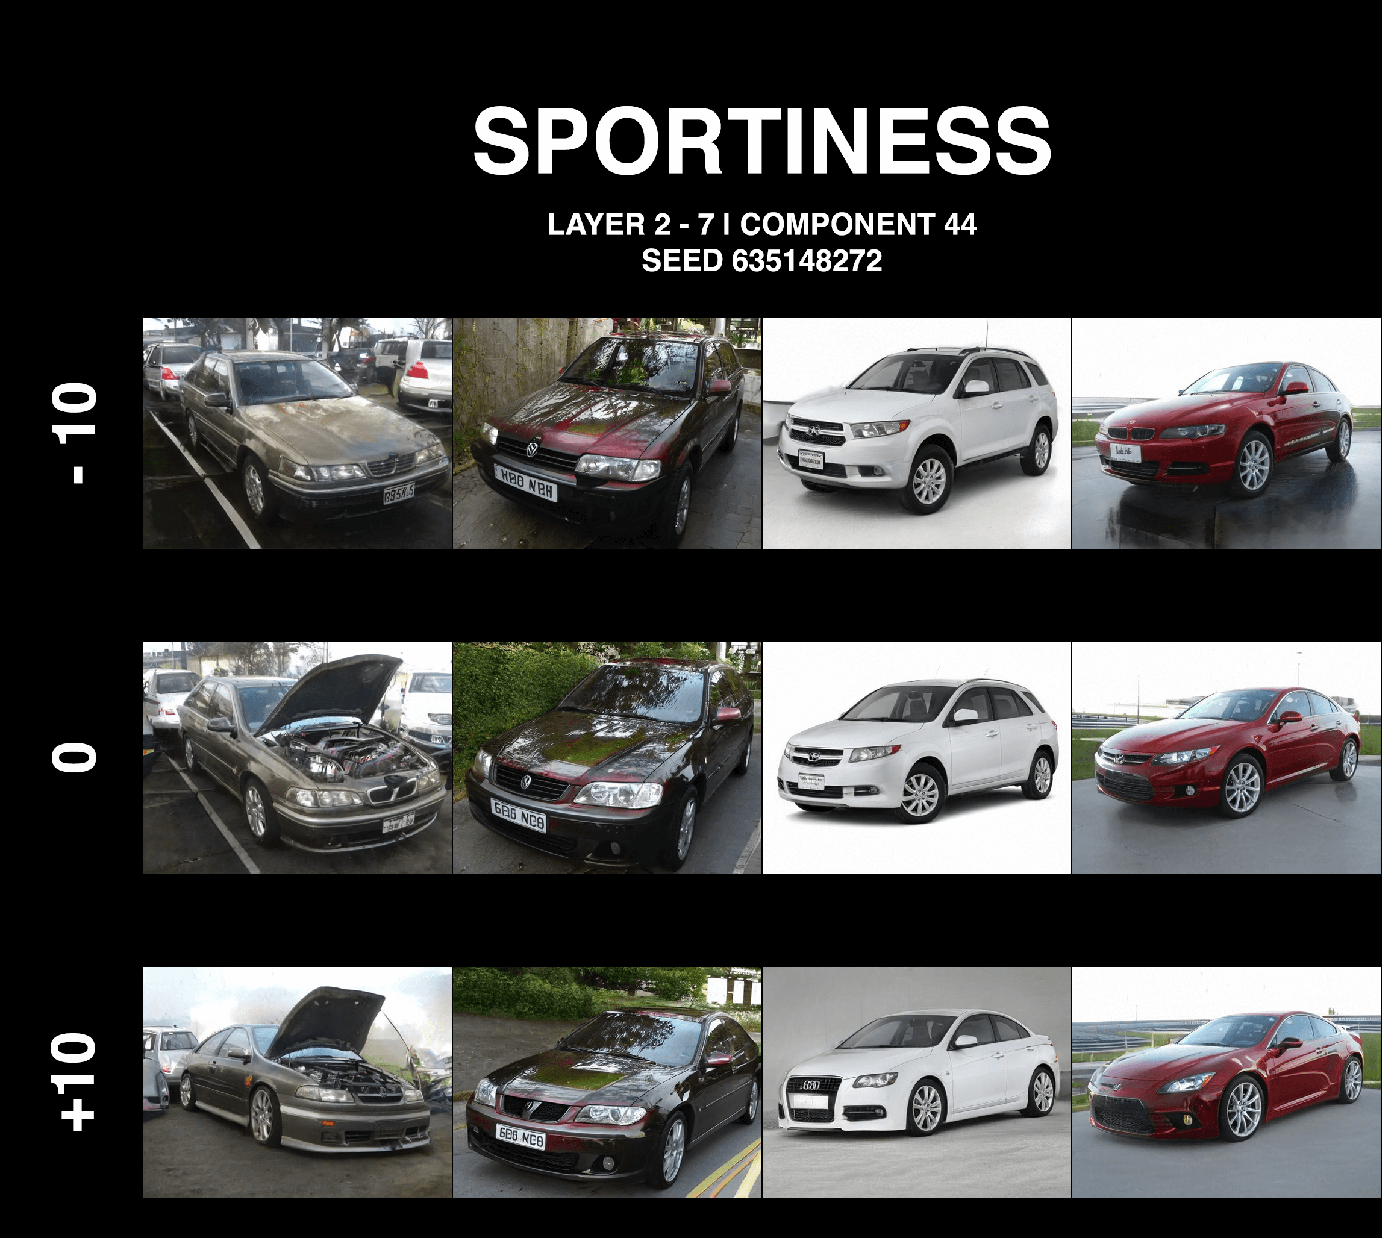
\includegraphics[width=\textwidth]{images/Sportiness.pdf}
  \caption{Major edits}
  \label{fig:sportiness}
\end{subfigure}
\hspace{.02\textwidth}
\begin{subfigure}{.3\textwidth}
  \centering
  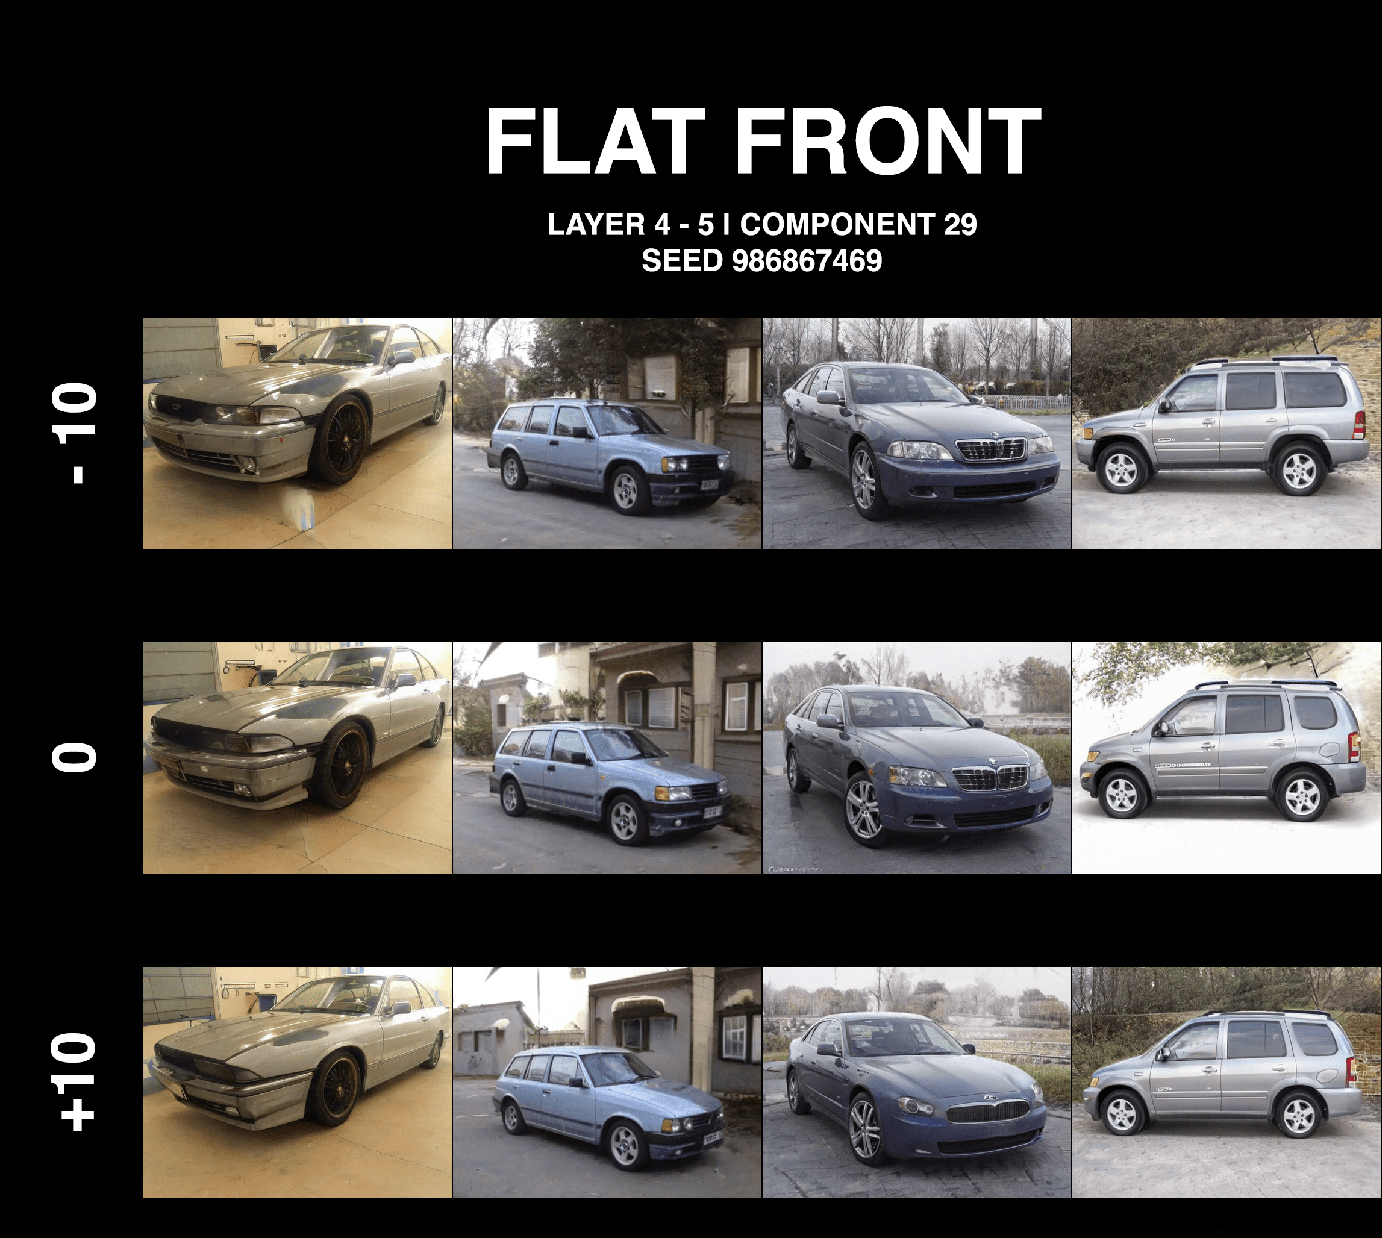
\includegraphics[width=\textwidth]{images/flat_front.pdf}
  \caption{Major edits}
  \label{fig:flatfront}
\end{subfigure}
\captionsetup{width=.85\linewidth}
\captionsetup{justification=centering}
\caption{Some of the grouped images used for external evaluation. Note that the textual description was removed when shown to the participant.}
\label{fig:groupedsurvey}
\end{figure*}

\begin{figure*}
\centering
\begin{subfigure}{.3\textwidth}
  \centering
  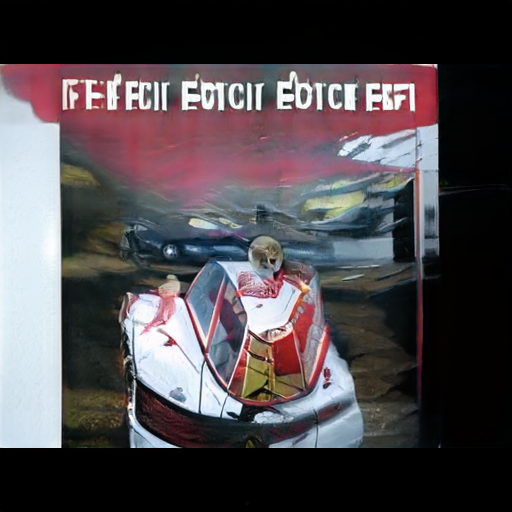
\includegraphics[width=\textwidth]{images/single1.png}
  \caption{Creative artefact}
  \label{fig:survey_creative_artefact}
\end{subfigure}%
\hspace{.02\textwidth}
\begin{subfigure}{.3\textwidth}
  \centering
  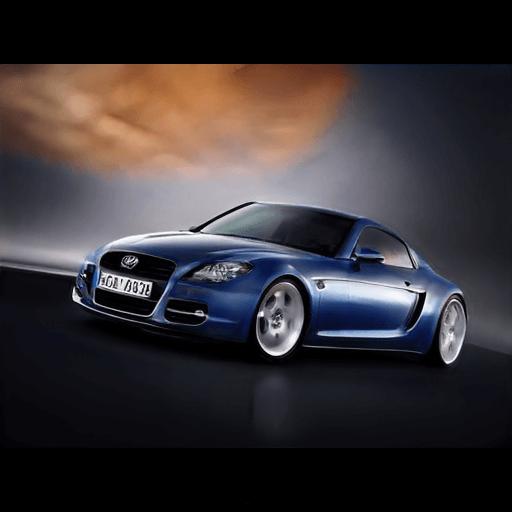
\includegraphics[width=\textwidth]{images/single6.png}
  \caption{Very realistic}
  \label{fig:survey_realistic}
\end{subfigure}
\hspace{.02\textwidth}
\begin{subfigure}{.3\textwidth}
  \centering
  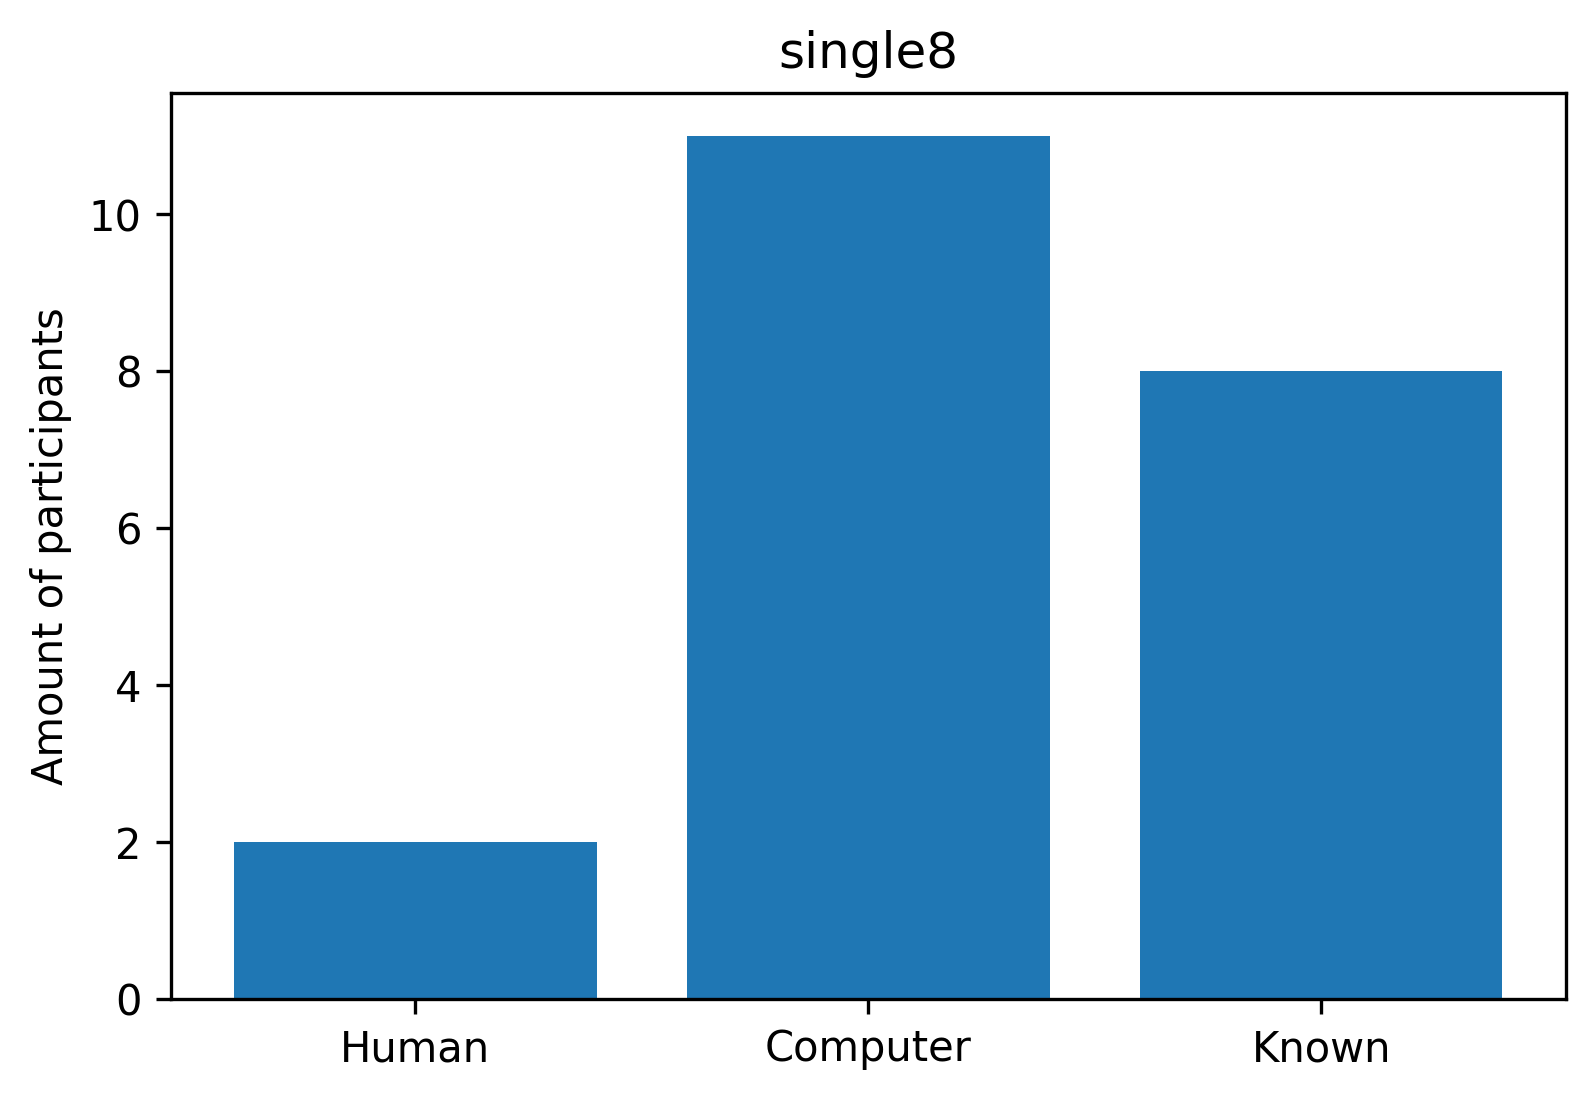
\includegraphics[width=\textwidth]{images/single8.png}
  \caption{Challenging angle}
  \label{fig:survey_angle}
\end{subfigure}

\vspace{.02\textwidth}

\begin{subfigure}{.3\textwidth}
  \centering
  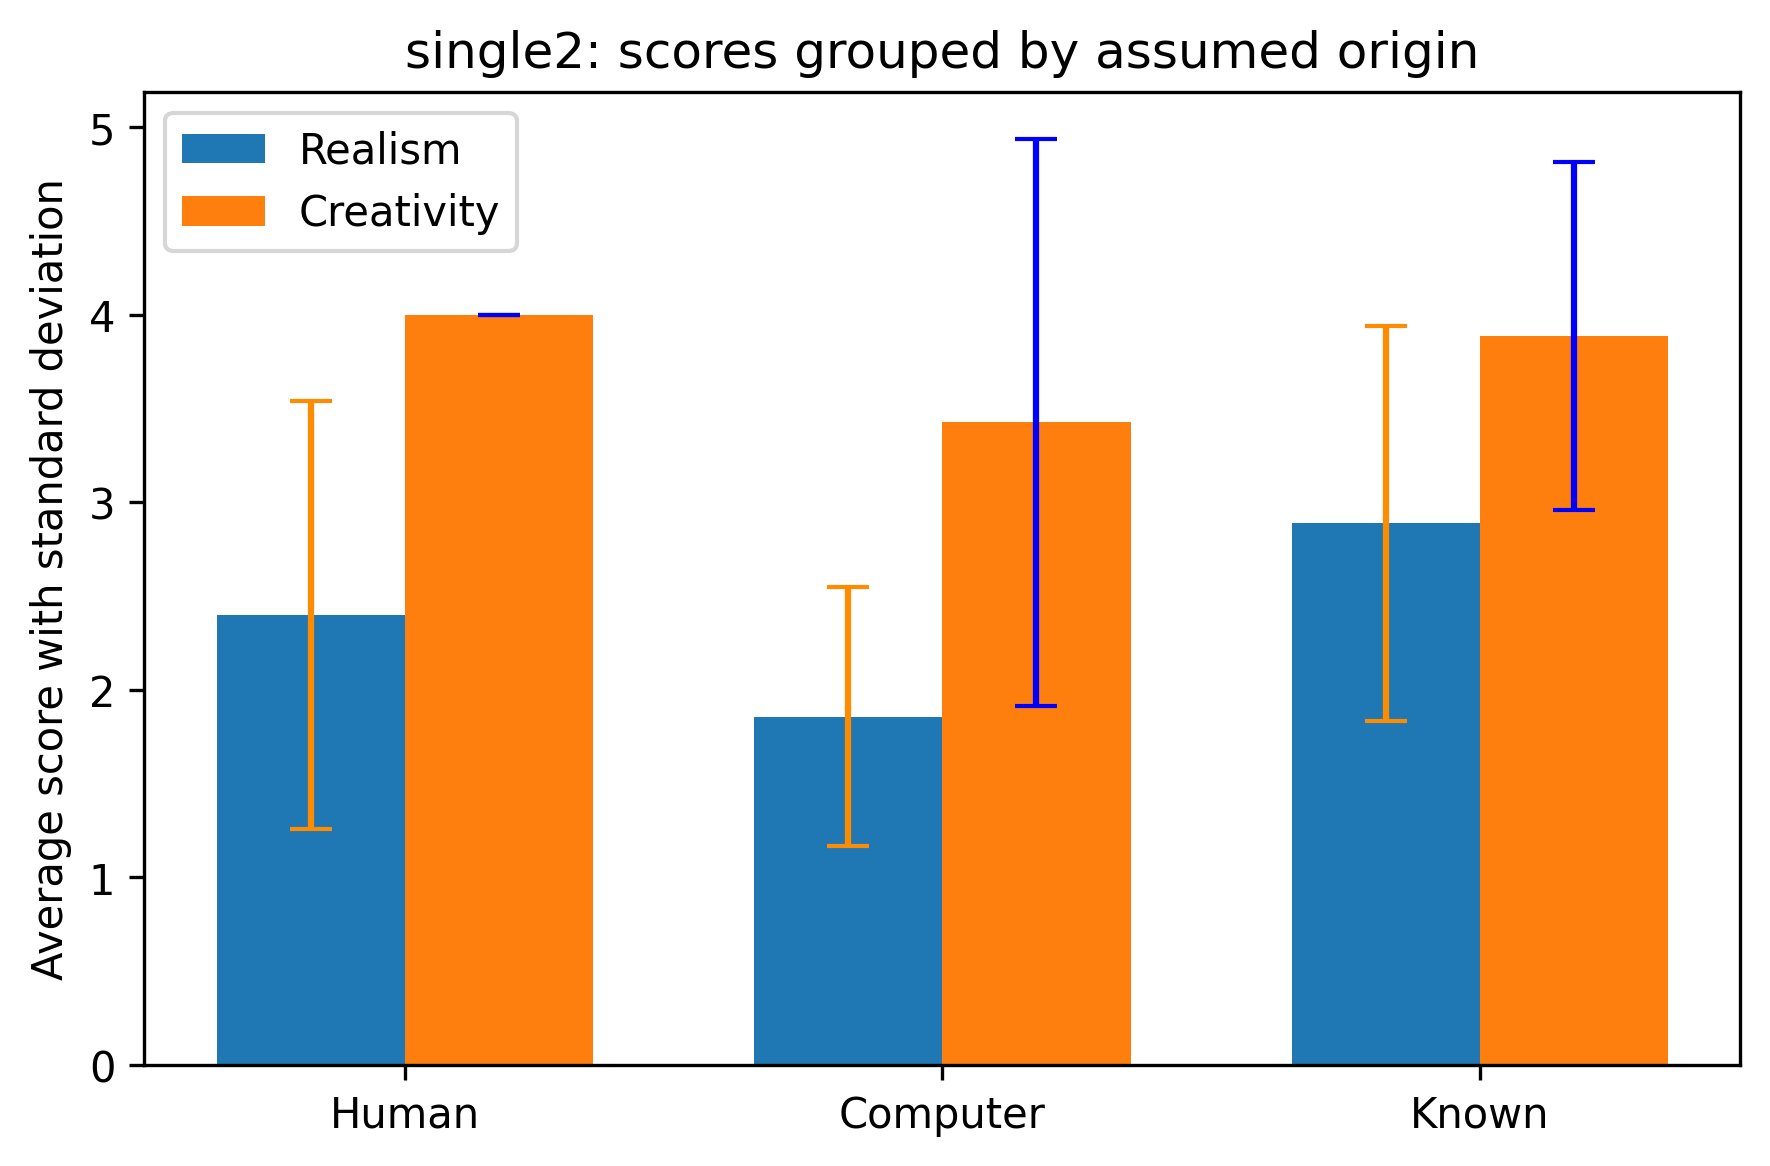
\includegraphics[width=\textwidth]{images/single2.png}
  \caption{Double front}
  \label{fig:survey_doublefront}
\end{subfigure}%
\hspace{.02\textwidth}
\begin{subfigure}{.3\textwidth}
  \centering
  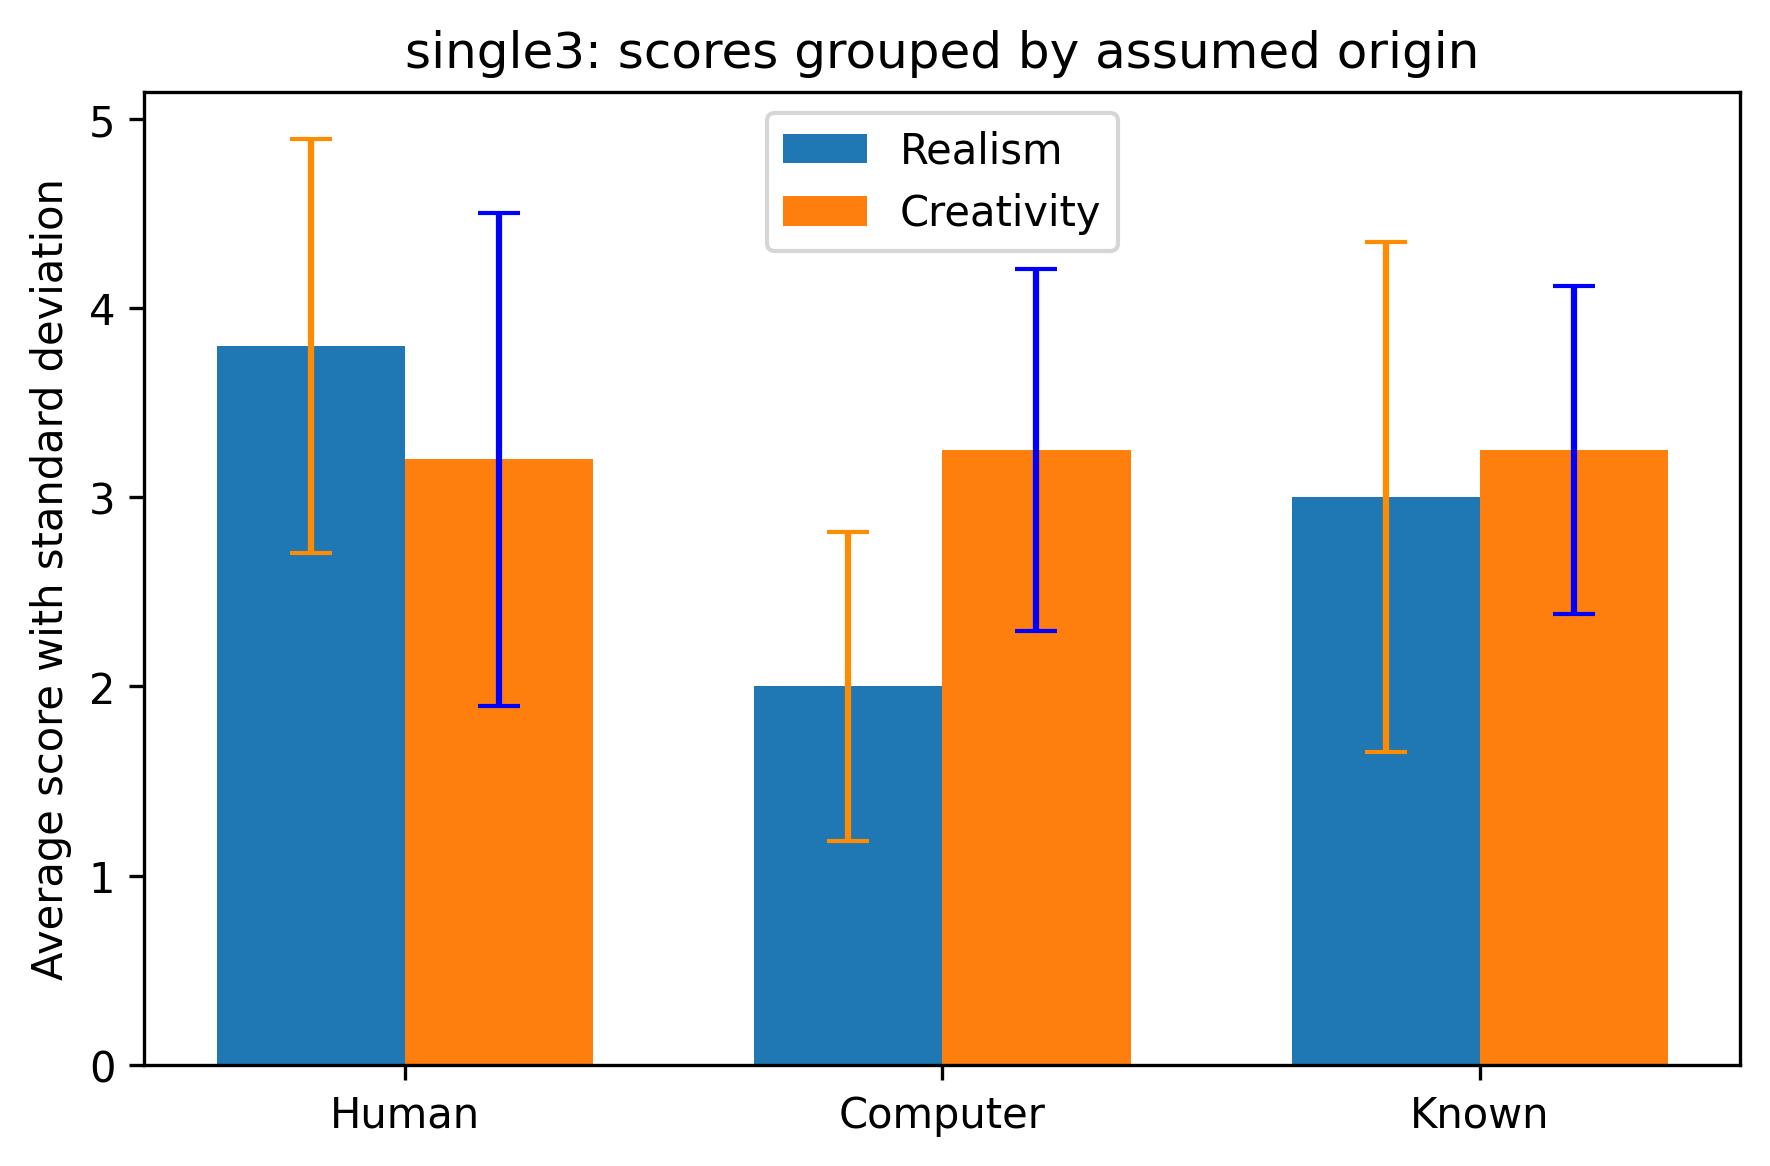
\includegraphics[width=\textwidth]{images/single3.png}
  \caption{Missing piece}
  \label{fig:survey_missing}
\end{subfigure}
\hspace{.02\textwidth}
\begin{subfigure}{.3\textwidth}
  \centering
  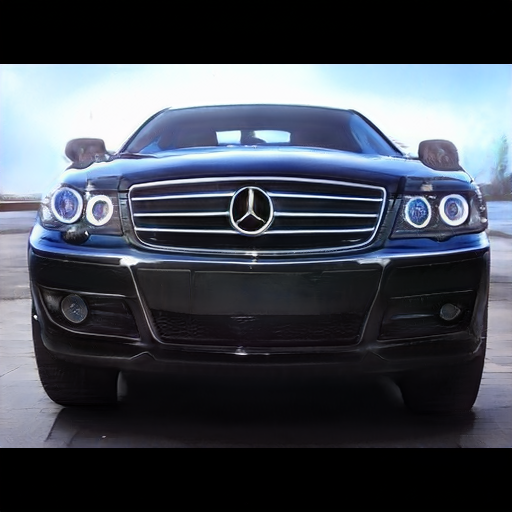
\includegraphics[width=\textwidth]{images/single4.png}
  \caption{Mercedes/BMW merge}
  \label{fig:survey_merged}
\end{subfigure}
\captionsetup{width=.85\linewidth}
\captionsetup{justification=centering}
\caption{Some of the single images used for external evaluation.}
\label{fig:singlesurvey}
\end{figure*}



%------------------------------------
\clearpage
\section{External evaluation results}
\label{sec:external_evaluation_results}

The external evaluation contains a lot of distinct rating criteria.
Since it wouldn't be feasible to analyse all of the results here, a Jupyter Notebook doing a complete analysis is made available under the results folder on the GitHub repository of this project \citep{github_project}.
Since the survey was quite lengthy and there were some minor bugs early on, it was expected not all of the participants registered completed the survey.
Indeed, after removing non-complete entrees the list of participants shrank from 32 to 21.
Of those 21 participants, 16 were male and 5 were female.
There were 7 participants with expertise, all of which were male.
Most of the participants belonged to the 20 years age group, one was colourblind and none had other vision problems.
These distributions seem healthy for a topic that is known to have more interest by men.

The Notebook then analyses the distribution of the creator assignments for each image.
The data shows that the random selection was successful and some images were highly assigned to either human or computer made.
Single images that were highly assigned to computer-generated were those containing non-realistic designs such as the one shown in figure \ref{fig:survey_creative_artefact} and \ref{fig:survey_angle}.
Interestingly enough, the grouped images that were highly assigned to computer-generated were those that contained minor edits such as the rim design edit shown in figure \ref{fig:rimdesign}.
This is interesting since those minor edits are harder for GANs, as they require the knowledge of smaller concepts from a car's design such as the wheel design.
The more realistic single images such as the one shown in figure \ref{fig:survey_realistic} were highly assigned to human-made.
For the grouped images, the major edits such as the one shown in figure \ref{fig:sportiness} were highly assigned to human-made as well.

\begin{figure*}
\centering
\begin{subfigure}{.45\textwidth}
  \centering
  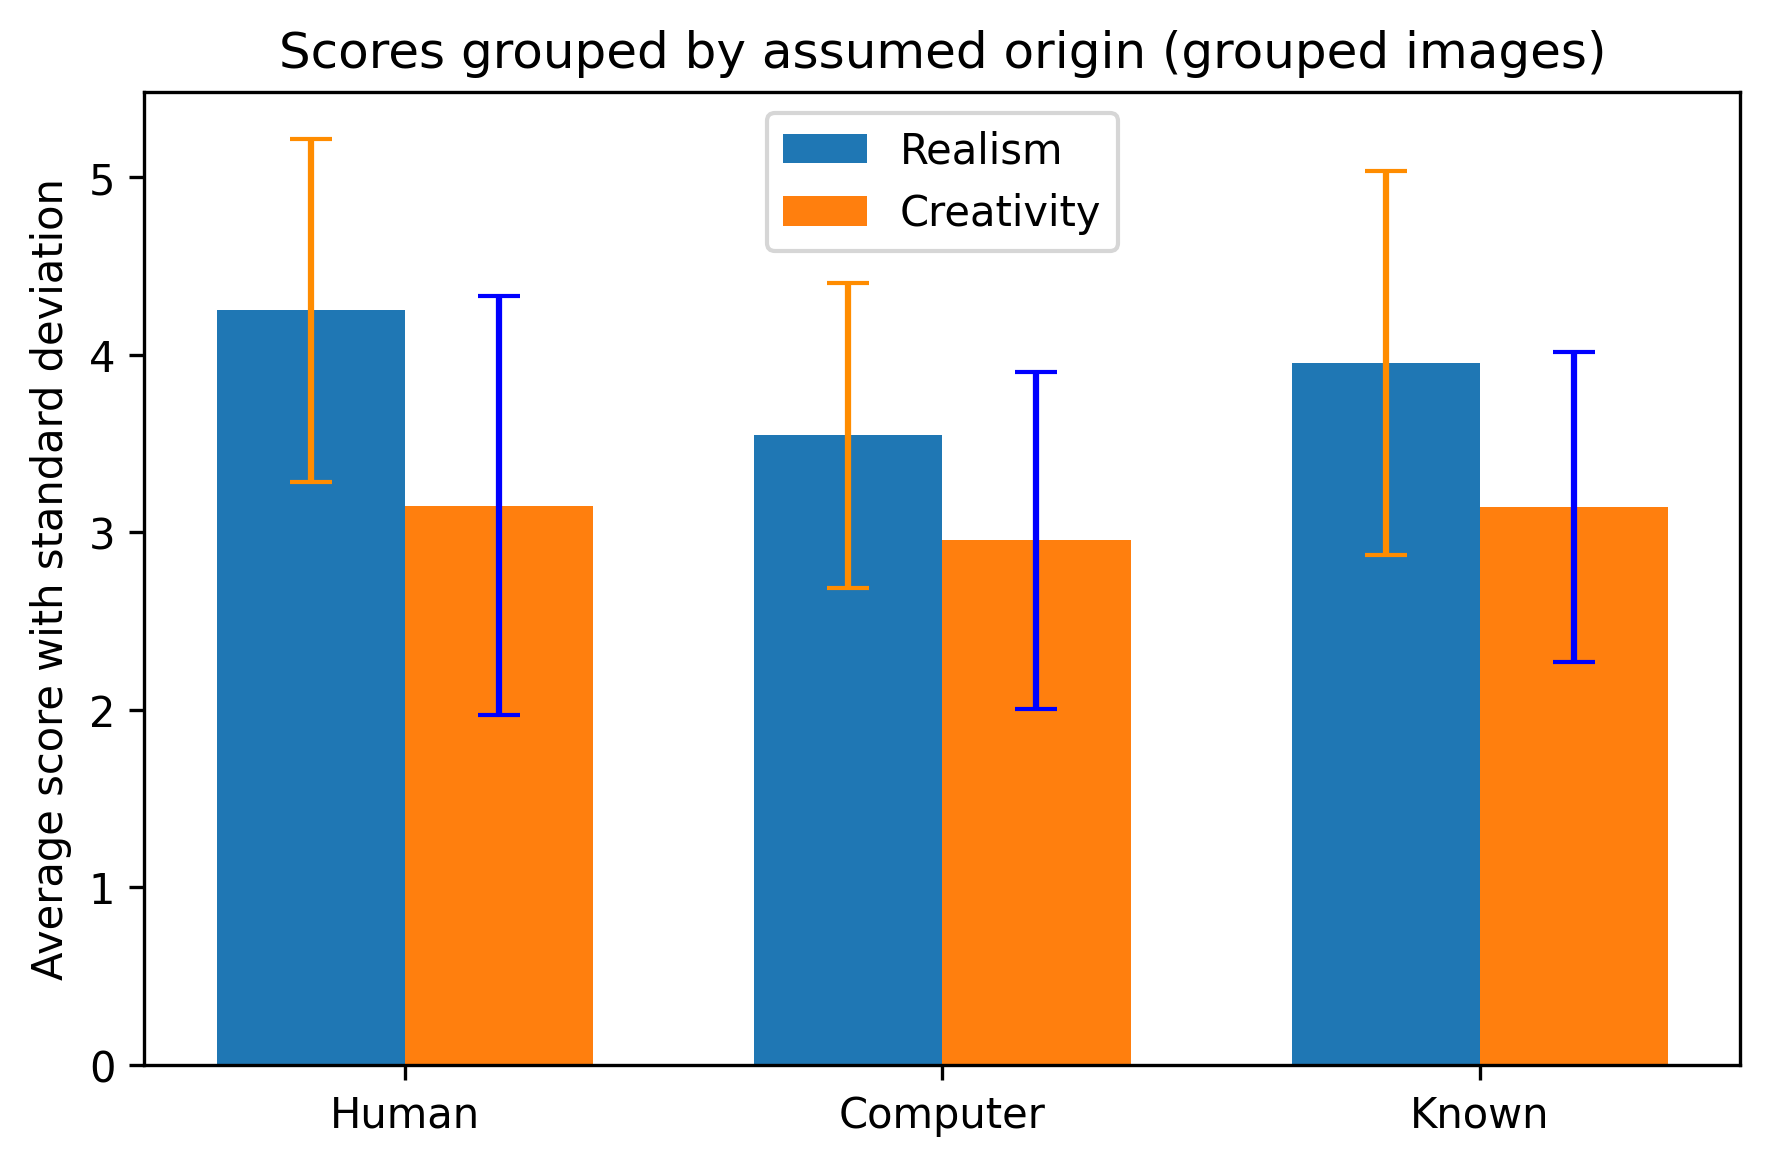
\includegraphics[width=\textwidth]{images/grouped_images_score_bias.png}
  \caption{Grouped image bias analysis}
  \label{fig:grouped_bias}
\end{subfigure}%
\hspace{.02\textwidth}
\begin{subfigure}{.45\textwidth}
  \centering
  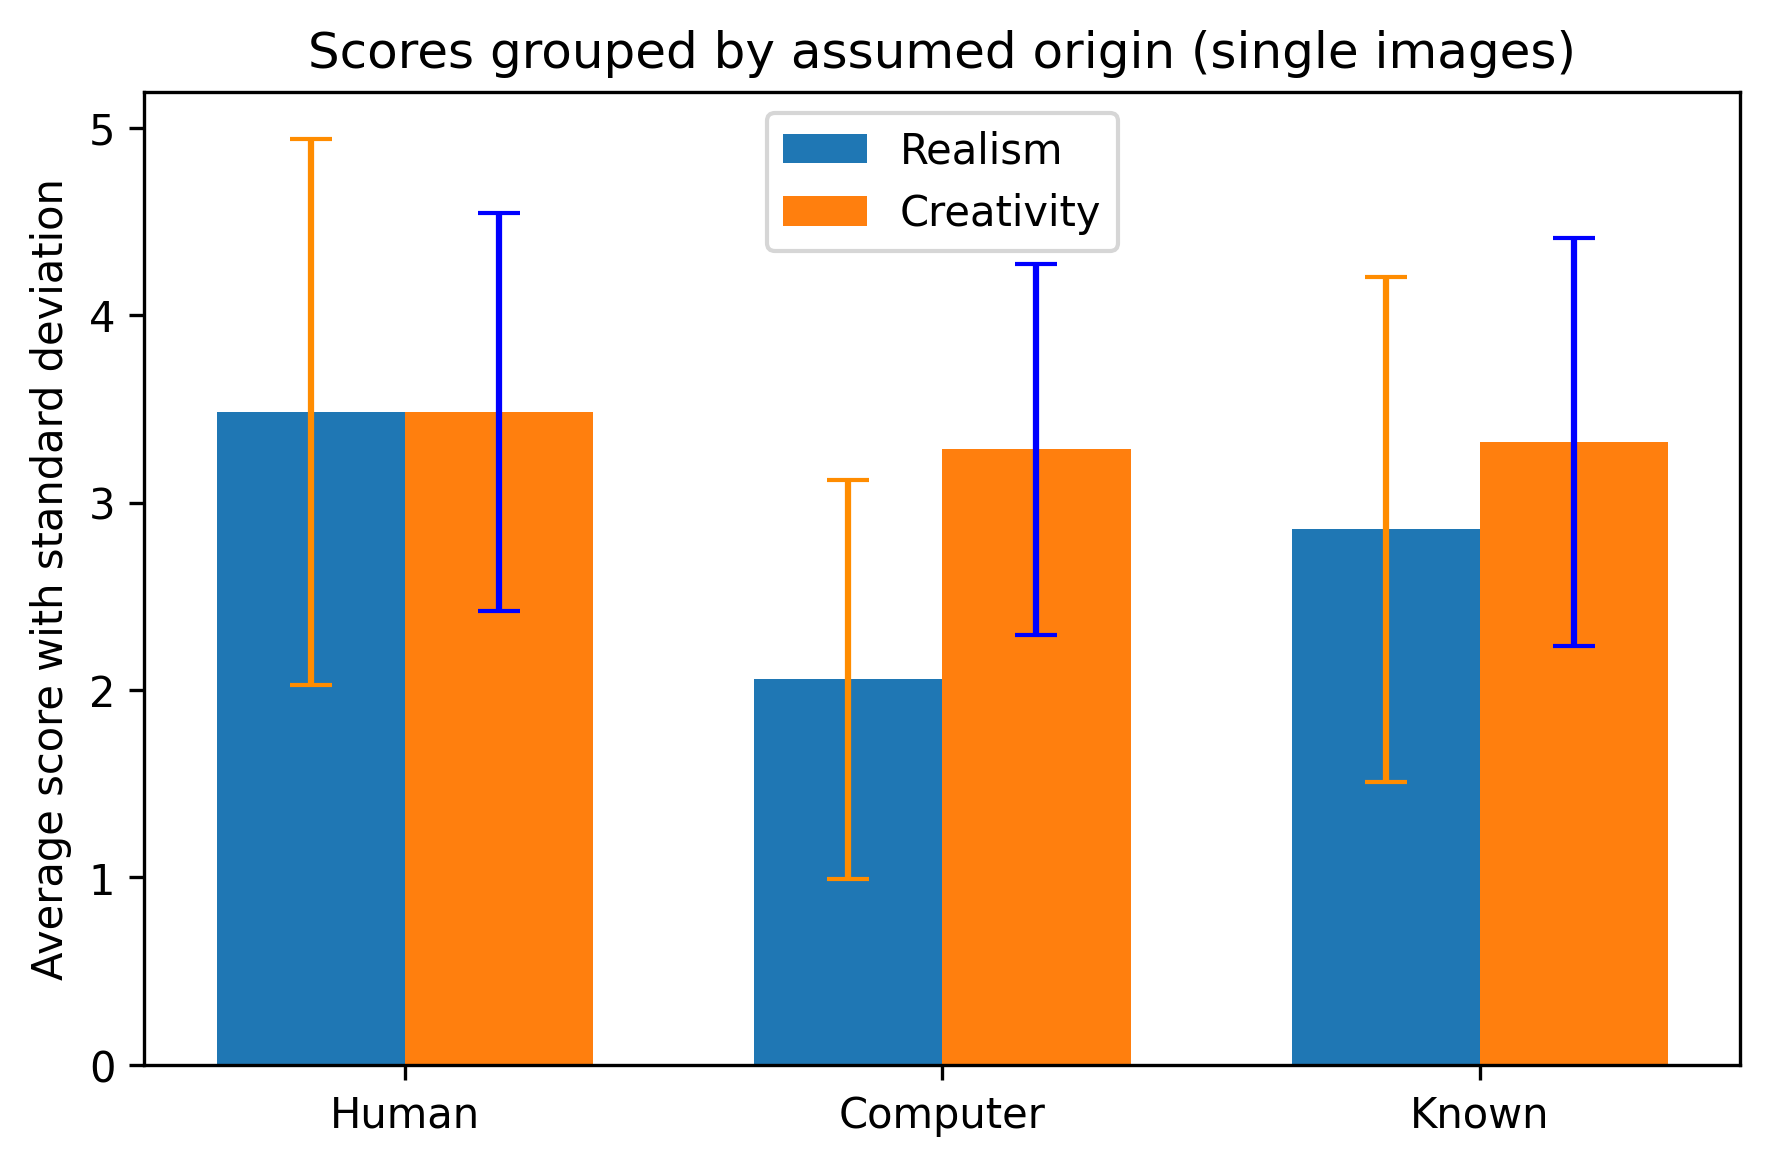
\includegraphics[width=\textwidth]{images/single_images_score_bias.png}
  \caption{Single image bias analysis}
  \label{fig:single_bias}
\end{subfigure}
\captionsetup{width=.85\linewidth}
\captionsetup{justification=centering}
\caption{ Bias analysis of grouped and single images. Analysis on a per image basis available on GitHub in the results Jupyter Notebook \citep{github_project}. }
\label{fig:bias}
\end{figure*}

This initial look at the results hints that the participants were biased in assigning shocking designs and minor edits to computers whilst assigning high-quality design and major edits to humans.
To validate this, the assigned realism and creativity scores were analysed per image, grouped by the assumed origin of the picture.
These analytics revealed it was indeed the case scores of human thought design were higher for both realism and creativity than when they were assigned to computer-generated.
More surprising, it became clear that after knowing that all designs were made by computers, this negative bias towards computer-generated design got slightly less. 
It is noted that most of these differences are small and for some images not statistically significant.

Figure \ref{fig:bias} summarizes these bias findings by showing the average score and standard deviation for realism and creativity grouped per thought origin.
Whilst it is concluded from these results that a bias against computer-generated design is present, only 6 out of 21 participants thought they were biased.
Interesting notes on this included "[...] I might have assigned the broken looking ones to pc" and "[...] A few images were shockingly good. Very impressive stuff.".

\begin{figure*}
\centering
\begin{subfigure}{.45\textwidth}
  \centering
  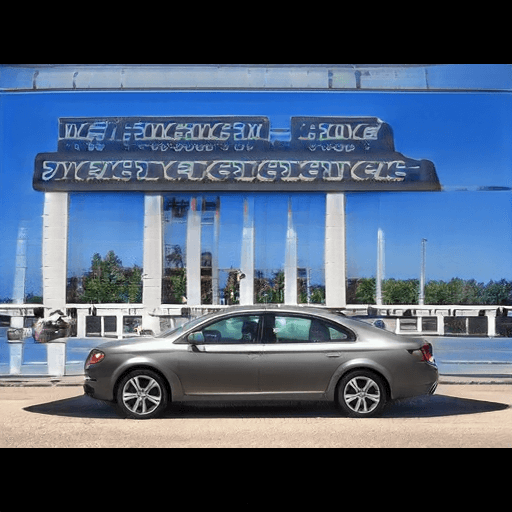
\includegraphics[width=\textwidth]{images/text.png}
  \caption{Generated car}
  \label{fig:similarcar_gan}
\end{subfigure}%
\hspace{.02\textwidth}
\begin{subfigure}{.45\textwidth}
  \centering
  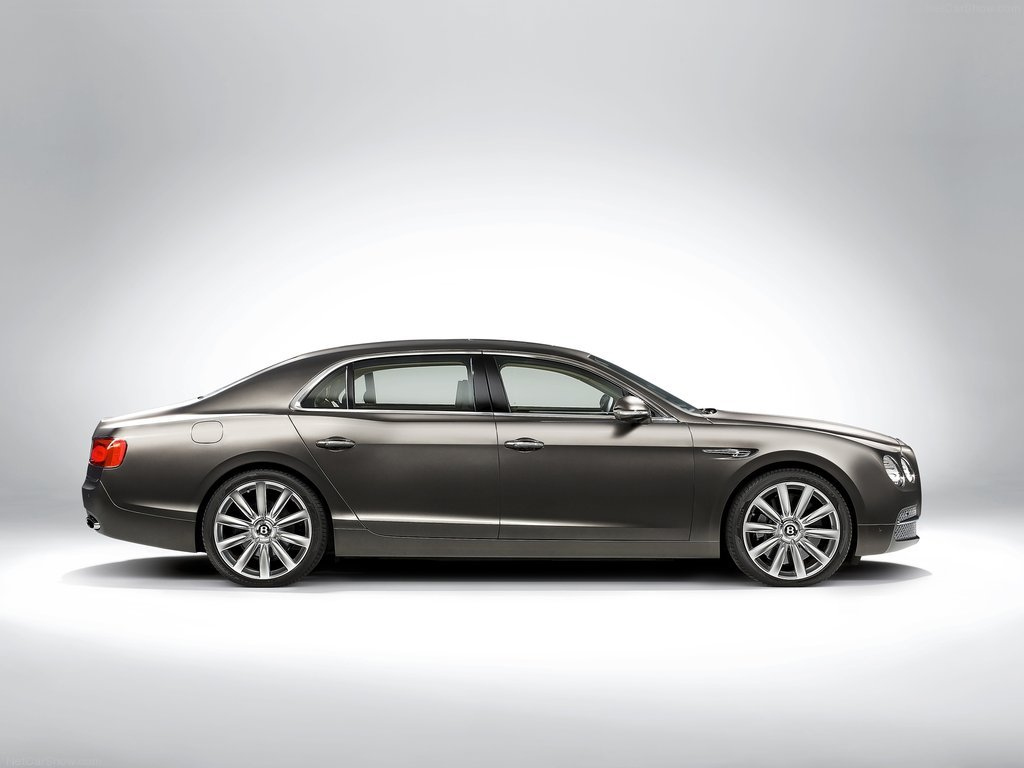
\includegraphics[width=\textwidth]{images/bentley-flying-spur.jpg}
  \caption{Bentley Flying Spur}
  \label{fig:similarcar_real}
\end{subfigure}
\captionsetup{width=.85\linewidth}
\captionsetup{justification=centering}
\caption{ Image of car generated by the GAN and the similar looking existing variant according to a participant. }
\label{fig:similarcar}
\end{figure*}

Since the notes from the bias gave an interesting insight into the participants' perception of the creative system, it was decided to have a look at the notes for the ratings similarly.
The most reoccurring notions from these notes are listed in what follows.
Be aware that these are generalisations of the received notes as no two notes are identical.
\begin{itemize}
    \item Notes that reoccurred on several images:
    \begin{itemize}
        \item "If it is computer-generated, it fooled me well."
        \item "[...] but weird artefact where [...]"
        \item "[...] these small changes make me give it a low creativity score." 
        \item "Reminds me of $<$car brand$>$."
        \item "[...] creative [...] not really a car [...]"
        \item "Don't really see a lot of difference." (grouped images with minor edits)
        \item "Look like completely different cars." (grouped images with major edits)
    \end{itemize}
    \clearpage
    \item Notes that reoccurred for specific grouped images:
    \begin{itemize}
        \item "[...] changed wheels [...]" (grouped image shown in figure \ref{fig:rimdesign})
        \item "[...] lowered [...] changed bumper [...] more sporty [...]" (grouped image shown in figure \ref{fig:sportiness})
        \item "[...] makes the car red [...]" (grouped image of flashy color modification)
        \item "[...] boxy [...] nose changes [...] (grouped image shown in figure \ref{fig:flatfront})
    \end{itemize}
    \item Notes that reoccurred for specific single images:
    \begin{itemize}
        \item "[...] looks nothing like a car [...] unique and creative [...] horror movie [...] album art [...]" (single image shown in figure \ref{fig:survey_creative_artefact})
        \item "[...] wow [...] interesting concept [...] weird thing with doors [...]" (single image shown in figure \ref{fig:missingpiece})
        \item "[...] Mercedes SUV [...] BMW headlights [...]" (single image shown in figure \ref{fig:survey_merged})
        \item "[...] cool text [...] Bentley Flying Spur [...]" (single image, comparison shown in figure \ref{fig:similarcar})
        \item "[...] funny [...] looks like another car drove into this one [...] seems confused about angles [...]" (single image shown in \ref{fig:survey_angle})
    \end{itemize}
\end{itemize}


\begin{figure*}
\centering
\begin{subfigure}{.45\textwidth}
  \centering
  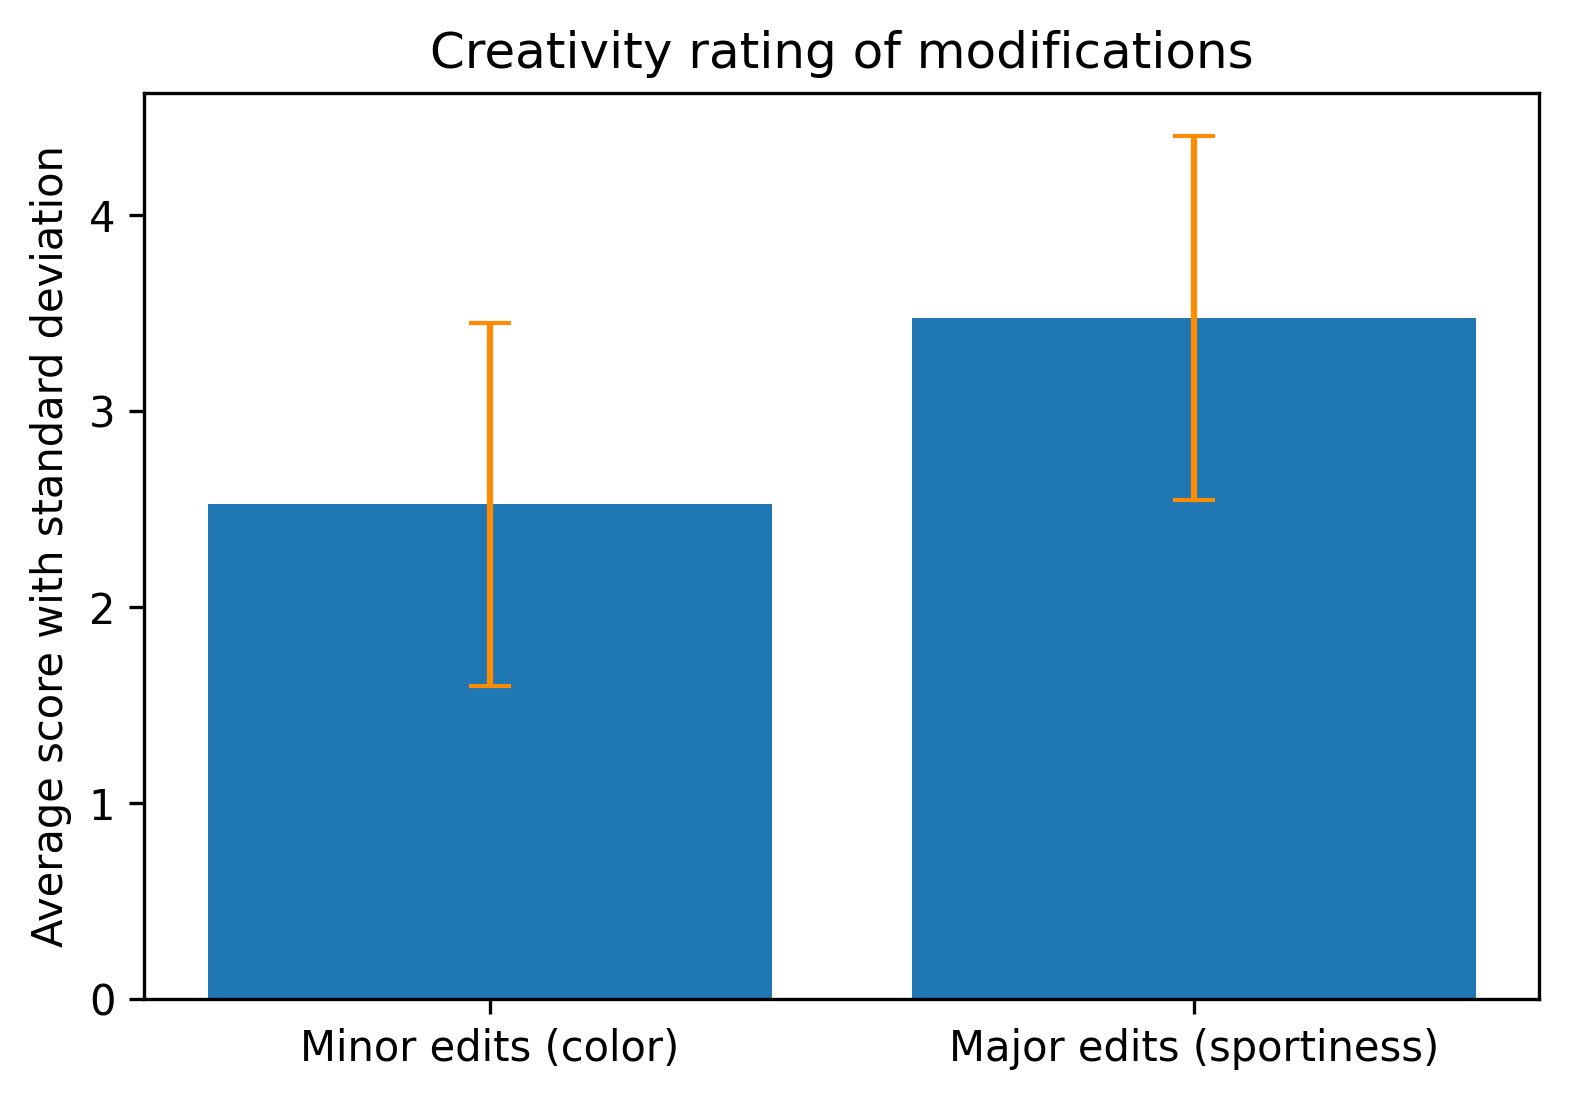
\includegraphics[width=\textwidth]{images/creativity_minor_changes.png}
  \caption{Creativity for modifications}
  \label{fig:creative_minor_changes}
\end{subfigure}%
\hspace{.02\textwidth}
\begin{subfigure}{.45\textwidth}
  \centering
  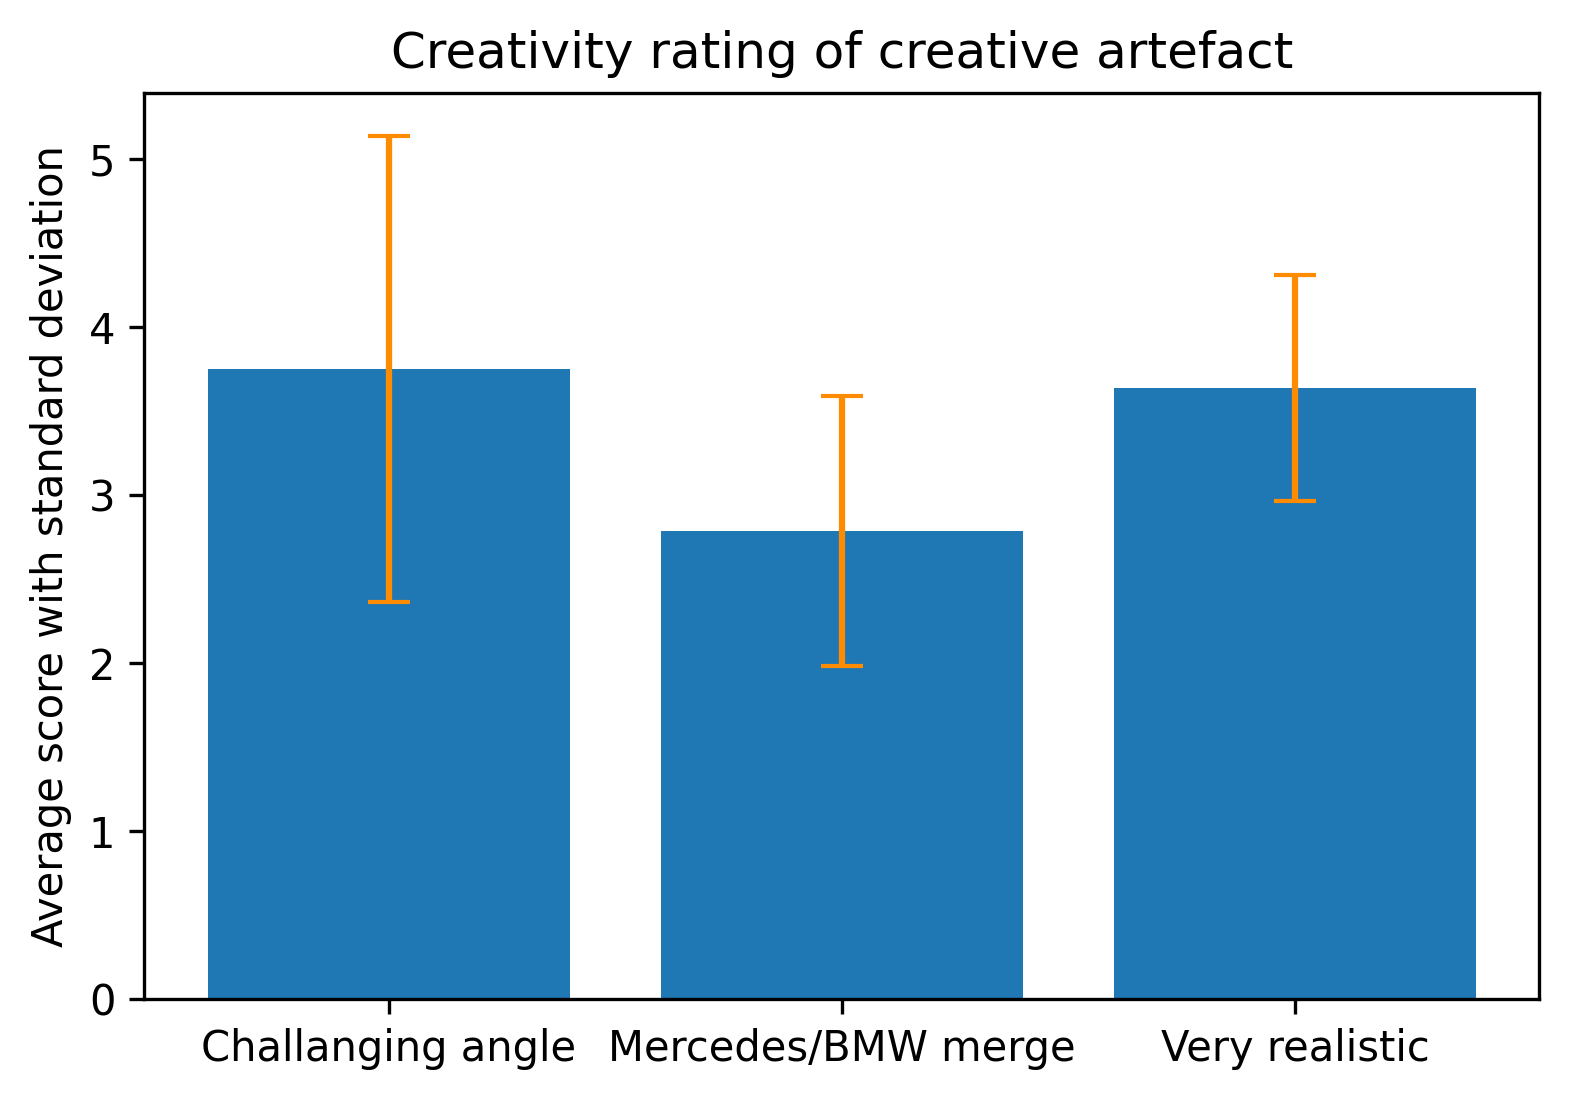
\includegraphics[width=\textwidth]{images/single_images_creativity.png}
  \caption{Creativity for single images}
  \label{fig:creative_single_images}
\end{subfigure}
\captionsetup{width=.85\linewidth}
\captionsetup{justification=centering}
\caption{Creativity rating comparisons based on type of image. Data from participants that knew it was machine made.}
\label{fig:creativity_statistics}
\end{figure*}

These notes give a good insight into the impressions of the participants.
It becomes apparent that the found concepts through GANSpace were also recognized by the participants.
Whilst, as already discussed, the possibility of doing minor edits through GANSpace is technically more impressive, it seems to be less impressive and creative to participants.
This can also be seen in figure \ref{fig:creative_minor_changes} where the creativity rating for the color modification and sportiness modification from figure \ref{fig:sportiness} are compared.
This hints that the "shocking" aspect of creativity seems to play an important role in the participants' ratings.
Indeed, when doing a similar comparison between the unrealistic challenging angle (figure \ref{fig:survey_angle}), a basic merge (figure \ref{fig:survey_merged}) and a very realistic (figure \ref{fig:survey_realistic}) car design, the more shocking designs get better ratings than the typical looking car.
The Jupyter Notebook then goes further by looking at the correlation matrix and more.
These extra analysis steps are not reported further as they don't teach much new information.
\chapter{Discussion}
\label{part:conclusions}

% NOT OK

With all major parts of the creative system discussed and the external evaluation results analysed, a conclusion on the results is given.
From this, a reflection on the designed system is given and the added value of this paper is discussed.
The paper ends by mentioning interesting future work and an important closing remark.


%------------------------------------
\section{Conclusions on the external evaluation}
\label{sec:conclusion_external_results}

The received ratings corresponded nicely with the intend of the images.
Artefacts of the system received high creativity scores but low ratings for the realism and car measure as they do not contain all required car components.
This makes them creative artefacts of the system that are interesting but not particularly useful for the domain.
Luckily these artefacts didn't occur often and would likely occur even less if the GAN were trained for even more epochs.

The system's learned concepts found through the extended GANSpace tool were also recognized by the participants, further confirming the labelling given for their role in the image generation.
The manual selection as replacement of the proposed similarity rating measure also proved successful since the only comparison to an existing car model was the one displayed in figure \ref{fig:similarcar}.
Whilst these cars do share similarities, they differ greatly when taking into account the similarities between designs in the domain.
It is not unlikely these two cars could co-exist in Bentley's car range. 
Many comments and mediocre ratings of similarity suggest this recognition of existing car brand styling traits occurs often.
Remember, this behaviour is often desired in the domain and thus positive for the system.

It is also shown that a generated car design can score great for reality, creativity and the other measure all at once.
With the car design shown in figure \ref{fig:survey_realistic} being the participant's favourite.
This generated design is indeed very intriguing, and thanks to the relatively realistic background it is not hard to imagine it being a press photo of a newly announced model.

The system is also capable of generating designs that can function as an inspiration for car designers even if they aren't perfect.
This was the case with the image shown in figure \ref{fig:missingpiece}.
The concept of a convertible truck is novel and whilst the image is not a perfect design due to missing pieces, it clearly shows the new concept and can be used as inspiration for car designers.




%------------------------------------
\section{Reflection on the developed creative system}
\label{sec:reflection_system}

The designed system is defended to be a creative system by explaining the different components based on Ventura's CC description paper as well as putting it into terms of the CSF.
The issues that GANs have to be accepted in the CC field were tackled, albeit mostly manual and not well generalisable for now.
However, the manual process can be automated and build into the proposed pipeline, given that there is enough computational power available.
These added measures don't limit the GANs capabilities as is also shown by this paper's system.
All of the different components are well documented and results can easily be recreated.
Readers are invited to play with the system and optimize it even further.

It isn't hard to imagine an optimized version of the system trained on a specific set of car models can function as an inspiration source for car designers.
This makes this creative system one that has clear potential in the industry as an aid for a creative profession rather than to replace it.
This is much like the system created by \citet{creativecargan}, which was made to optimize a car designers pipeline.
Since StyleGAN2 works so well for different types of image generation, it is also not hard to imagine a similar system being in place in different domains.
This would only require small changes to the proposed pipeline from figure \ref{fig:system_pipeline}.


%------------------------------------
\section{Added value}
\label{sec:added_value}

This paper discussed the shortcomings of GANs in the CC field.
By doing so, it also mentioned solutions that can be put in place to make GANs viable as creative systems.
These solutions were demonstrated in the creative system of this paper that is capable of generating novel car designs.
An external evaluation tool has been custom made and is available under the GPL V3 license.
This tool can be helpful for the CC field and other image evaluation settings. 


%------------------------------------
\section{Interesting future work}
\label{sec:future_work}

Some interesting future work has already been mentioned.
A summary is given below.
\begin{itemize}
    \item Train a StyleGAN2 model on a set of cars from one specific brand. Analyse the outputs together with a domain expert of that brand to further analyse the viability of such a system as an aid for a car designer.
    \item Implement the automatic similarity rating measure, ideally as part of the GAN and thus the training process.
    \item Implement a comparable system for a different domain, such as the clothing design domain.
    \item Perform an even broader external evaluation, possibly with car designers themselves.
\end{itemize}

%------------------------------------
\section{Closing remark}
\label{sec:closing_remark}

This paper made use of component analysis to discuss the system's capability of learning concepts.
This approach is widely used in literature to make deep NNs explainable.
An example of a paper that uses the same ideology is the mentioned paper by \citet{invidualunitanalysis}.
However, this approach is not without risk and a famous quote by E. Yudkowsky is given as a closing remark.


\epigraph{By far, the greatest danger of Artificial Intelligence is that people conclude too early that they understand it.}
{\textit{Eliezer Yudkowsky \\ AI theorist and writer}}

%references list
\nocite{*}
\printbibliography[heading=bibintoc, title={References}]
\end{document}
